% ----------------------------------------------------------
% Desenvolvimento
% ----------------------------------------------------------
\chapter{Desenvolvimento}\label{cap:desenvolvimento}
% ----------------------------------------------------------

% ----------------------------------------------------------
\section{Primeira Etapa - Estudo Prático das Tecnologias}\label{sec:primeira-etapa}
% ----------------------------------------------------------

O primeiro experimento realizado foi a tentativa de identificação de um \textit{beacon} com o \textit{RPi}, para o estudo de funcionamento e comportamento dessas tecnologias. Para isso, o ambiente foi configurado conforme \autoref{fig:inicio-ambiente}. 

\begin{figure}[htb]
	\caption{\label{fig:inicio-ambiente}Primeiro teste realizado, com \textit{RPi} e \textit{beacon MPact}}
	\begin{center}
		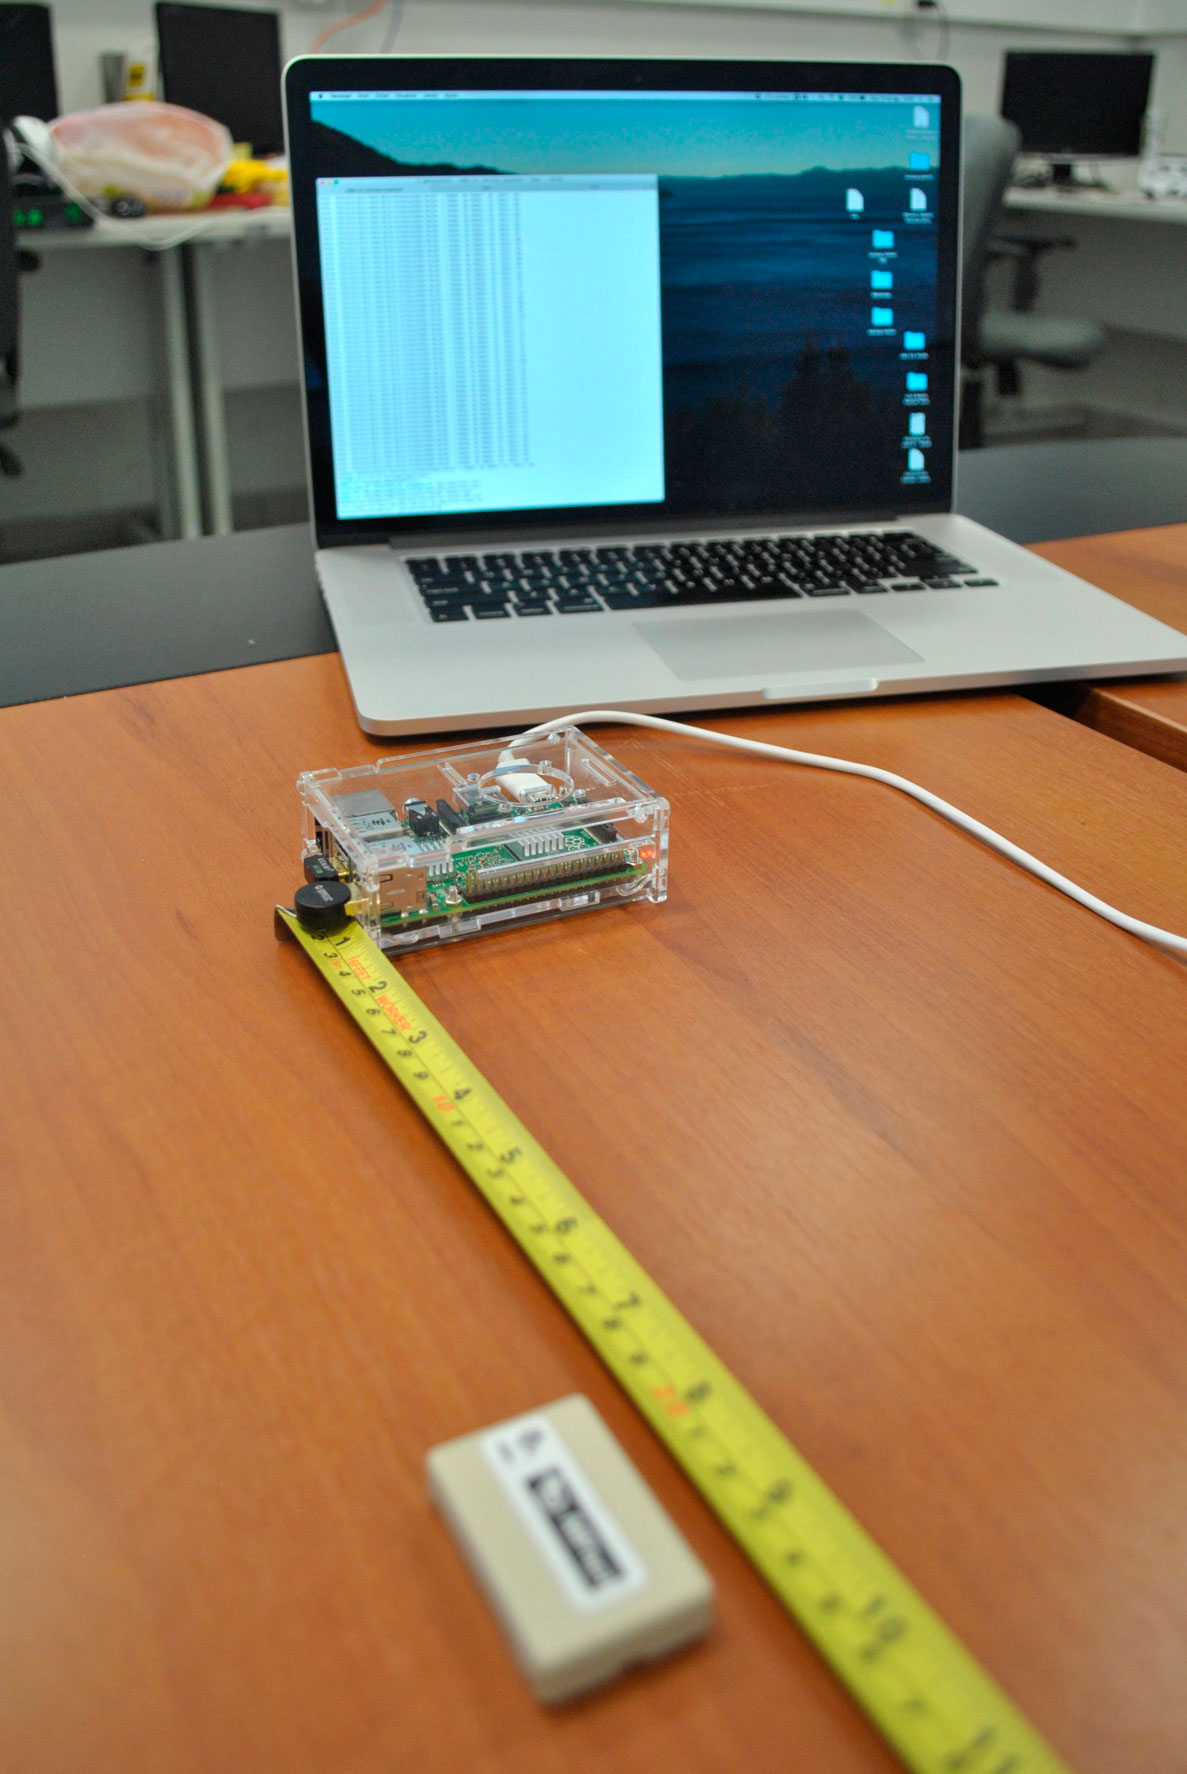
\includegraphics[width=0.66\textwidth]{img/ambiente1.jpg}
	\end{center}
	\legend{Fonte: elaborado pelo autor}
\end{figure}

O computador ficou conectado via SSH com o \textit{RPi}, recebendo as informações de leitura de pacotes \textit{BLE}. Os softwares utilizados para isso foram, conforme \citeonline{stack-overflow-ibeacon}, os seguintes:

\begin{alineas}
	\item \textbf{hcitool}: configurado da maneira \textit{hcitool lescan --duplicates}, faz um scan na frequência \textit{BLE} procurando por dispositivos que estejam transmitindo, conforme \autoref{fig:hcitool-lescan}.
	
	\begin{figure}[htb]
		\caption{\label{fig:hcitool-lescan}Software \textit{hcitool} executando}
		\begin{center}
			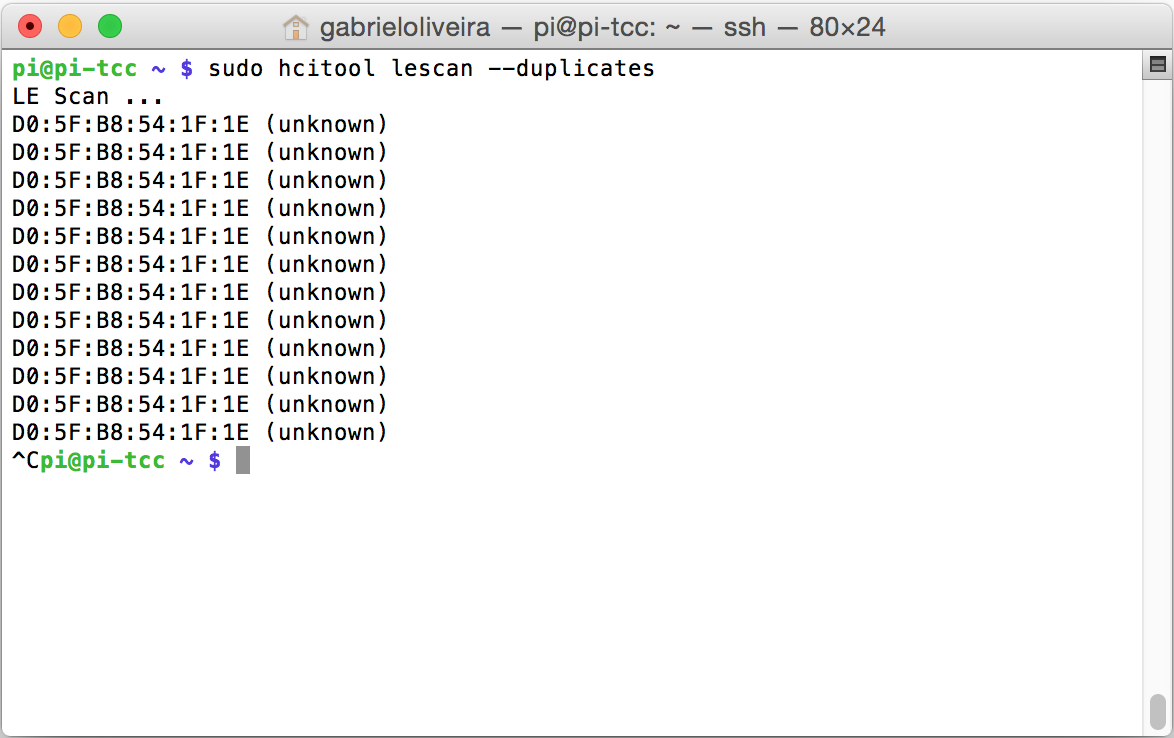
\includegraphics[width=0.6\textwidth]{img/hcitool-lescan.png}
		\end{center}
		\legend{Fonte: elaborado pelo autor}
	\end{figure}

	\item \textbf{hcidump}: em conjunto com o \textit{hcitool}, apresenta todos os pacotes escaneados na rede. Executado da maneira \textit{hcidump --raw}, conforme \autoref{fig:hcidump}.
	
	\begin{figure}[htb]
		\caption{\label{fig:hcidump}Software \textit{hcidump} executando}
		\begin{center}
			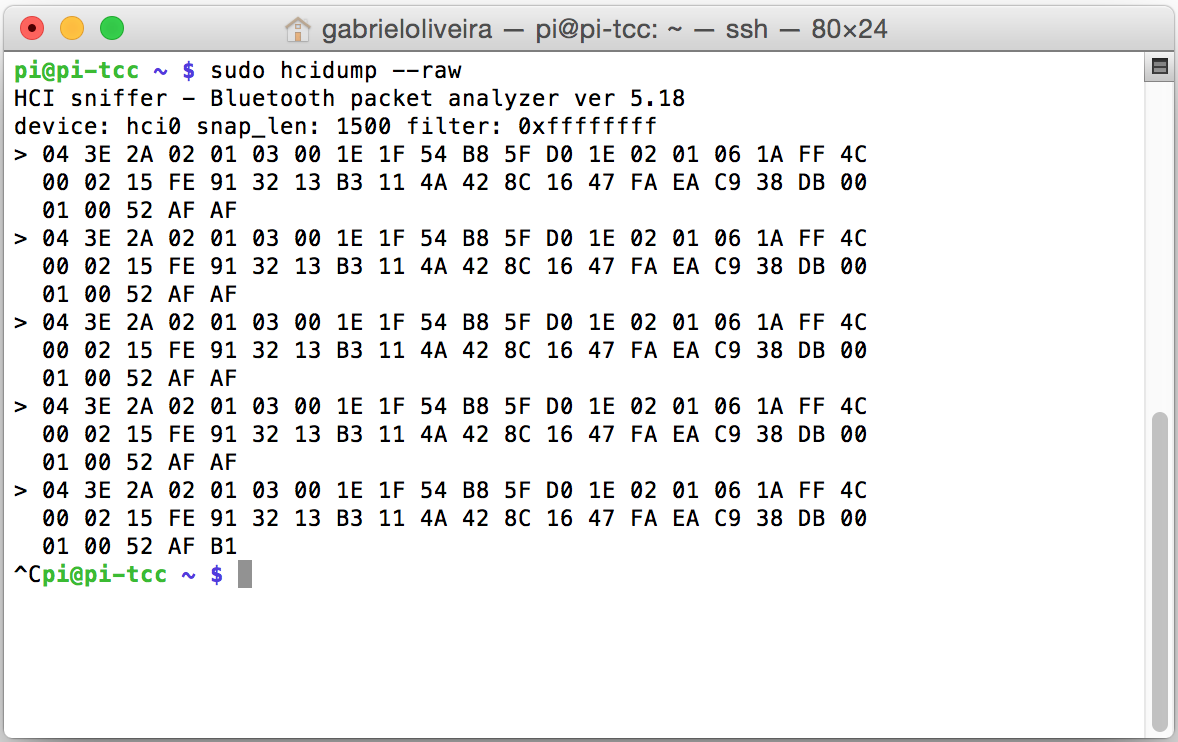
\includegraphics[width=0.6\textwidth]{img/hcidump.png}
		\end{center}
		\legend{Fonte: elaborado pelo autor}
	\end{figure}

\end{alineas}

Em seguida, com os softwares em execução e os pacotes sendo analisados, o \textit{beacon} foi movido ao longo mesa para ficar a diferentes distâncias do \textit{RPi}, conforme \autoref{fig:movimenta-beacon}. Esse passo foi necessário para verificar o formato dos pacotes recebidos e também analisar a distância máxima de identificação.

\begin{figure}[htb]
	\caption{\label{fig:movimenta-beacon}Teste com movimentação do \textit{beacon}}
	\begin{center}
		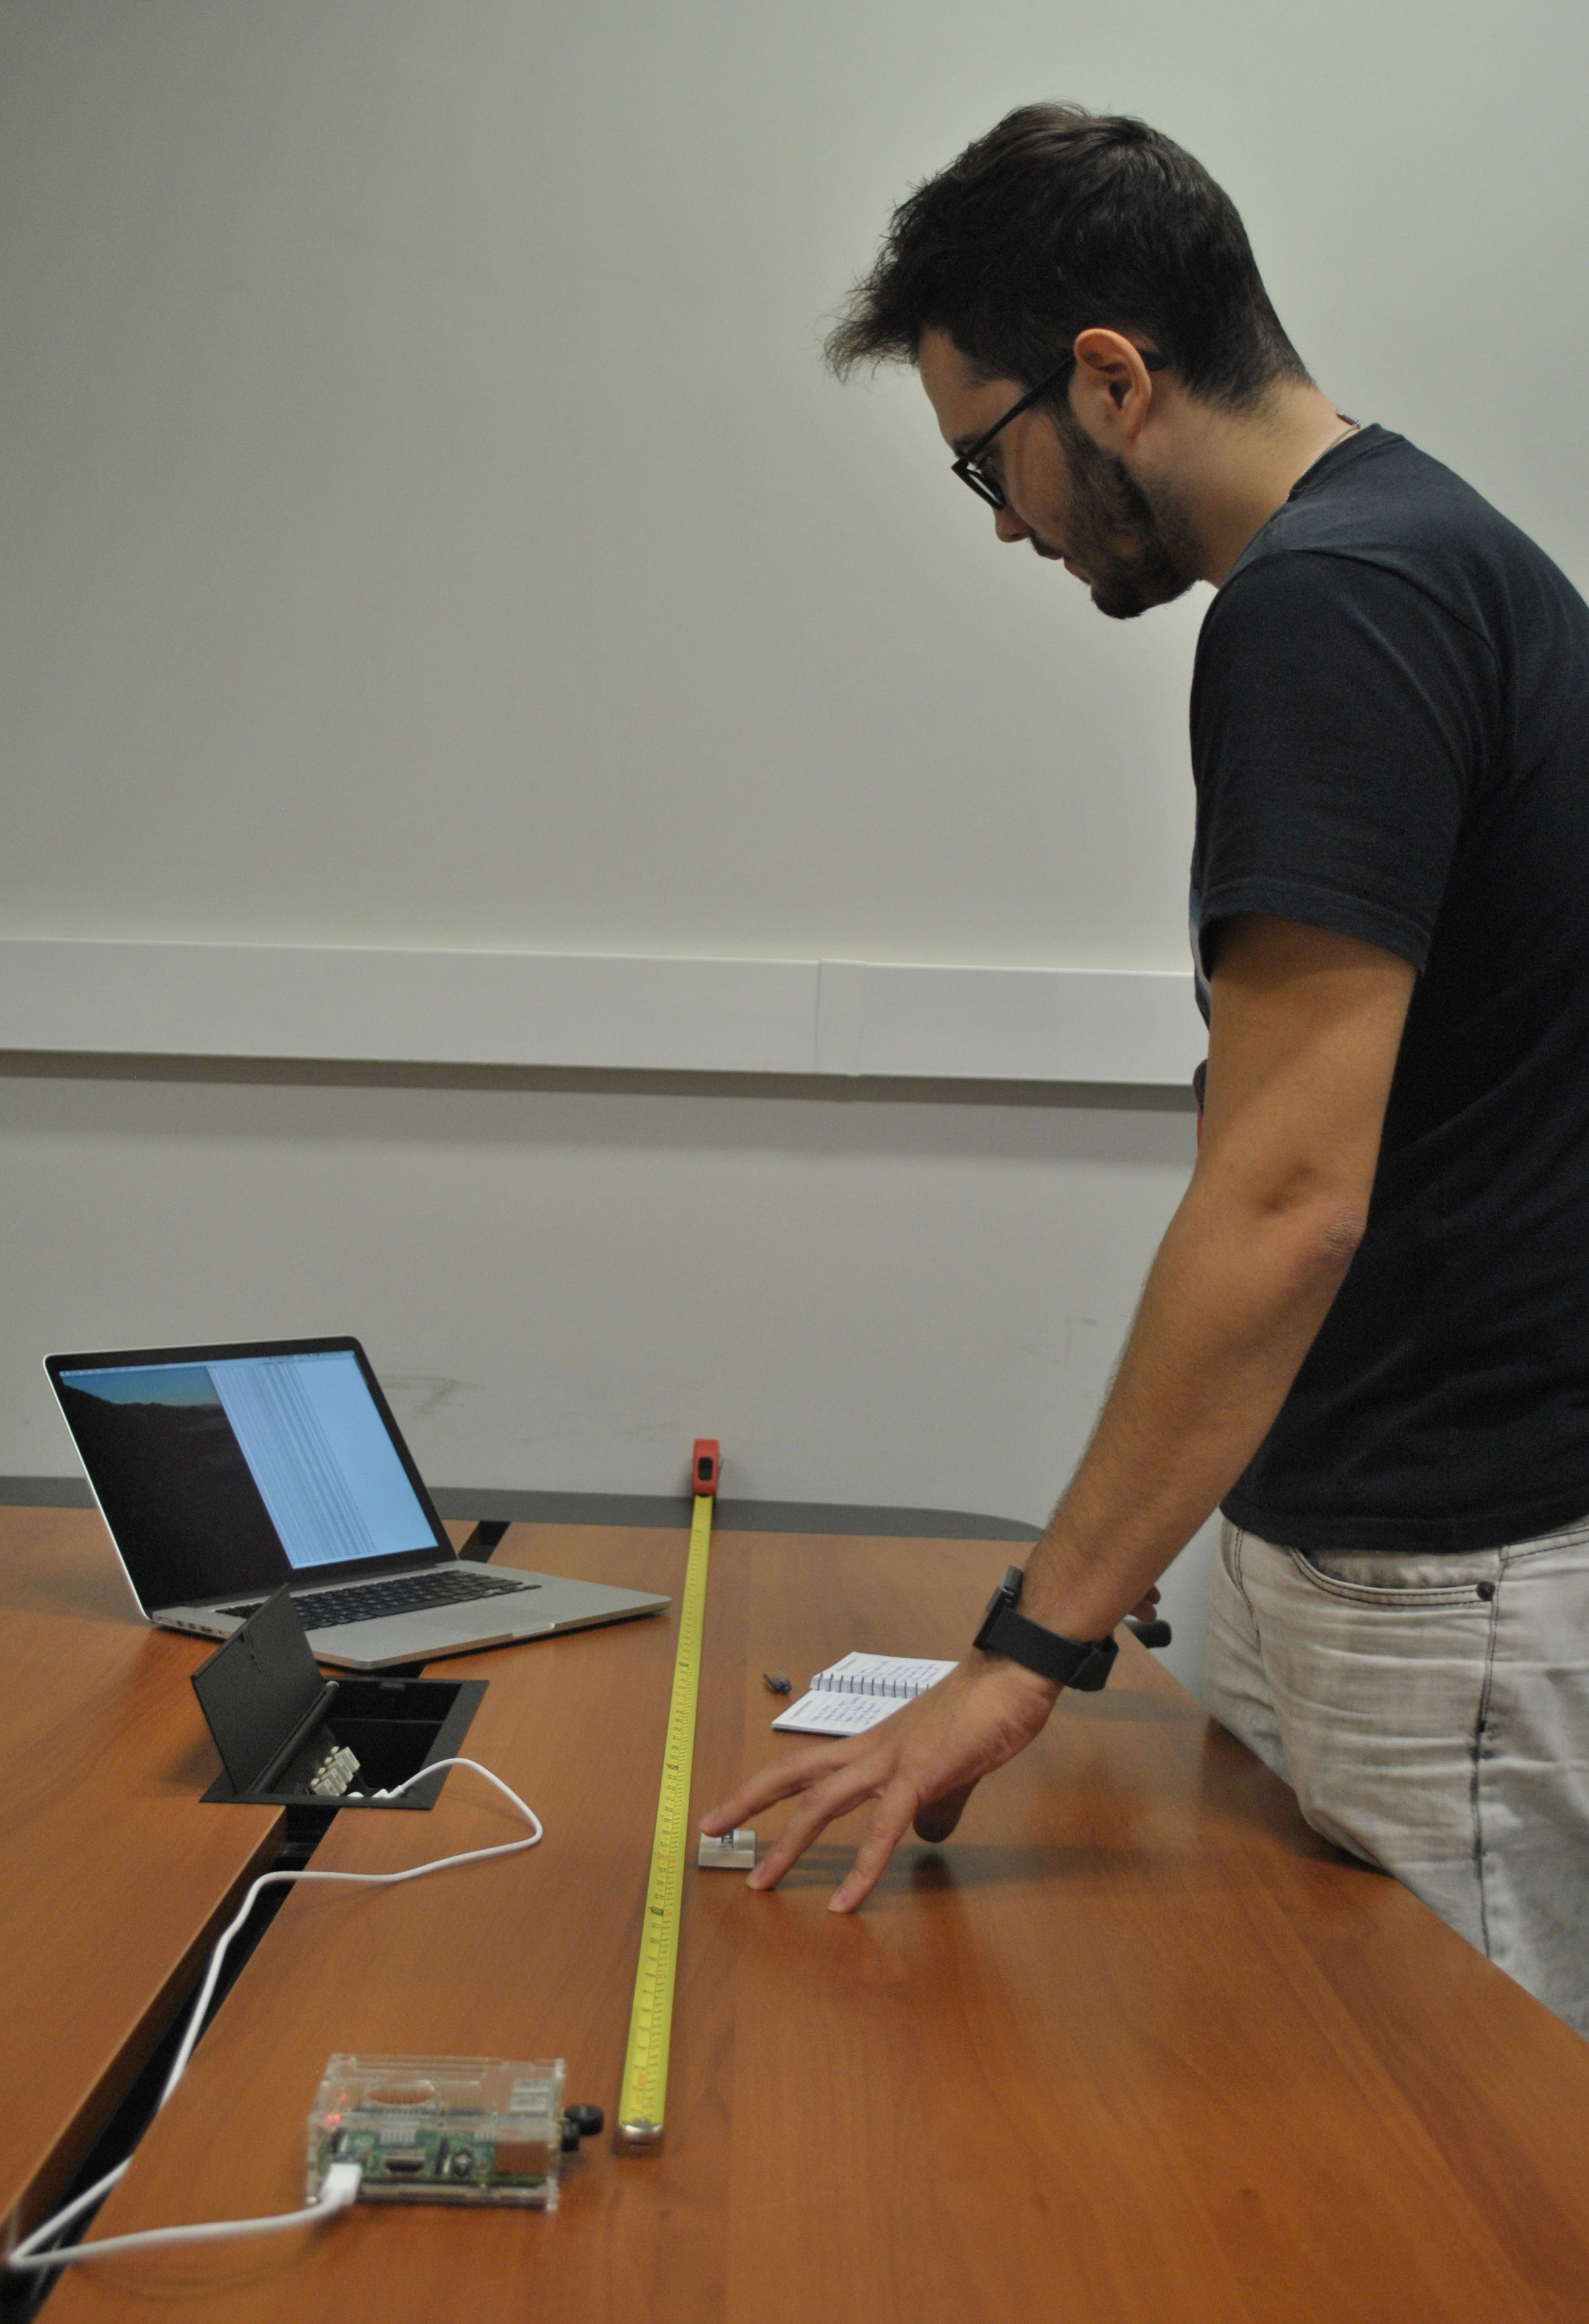
\includegraphics[width=0.7\textwidth]{img/ambiente4.jpg}
	\end{center}
	\legend{Fonte: elaborado pelo autor}
\end{figure}

Com o adaptador Orico BTA-406 e posicionamento na mesa conforme \autoref{fig:inicio-ambiente} e \autoref{fig:movimenta-beacon}, a cerca de 1,3 a 1,4 metros de distância entre o \textit{RPi} e o \textit{beacon} os pacotes já começaram a falhar e a leitura não foram tão constante.

O posicionamento do \textit{RPi} foi alterado para testes, conforme \autoref{fig:posiciona-rpi}. Notou-se uma melhoria na recepção dos pacotes, a 1,5 metros entre o \textit{RPi} e o \textit{beacon} os pacotes começaram a falhar, com recebimento de informações notada até 1,6 metros.

\begin{figure}[htb]
	\caption{\label{fig:posiciona-rpi}\textit{RPi} posicionado de outra maneira}
	\begin{center}
		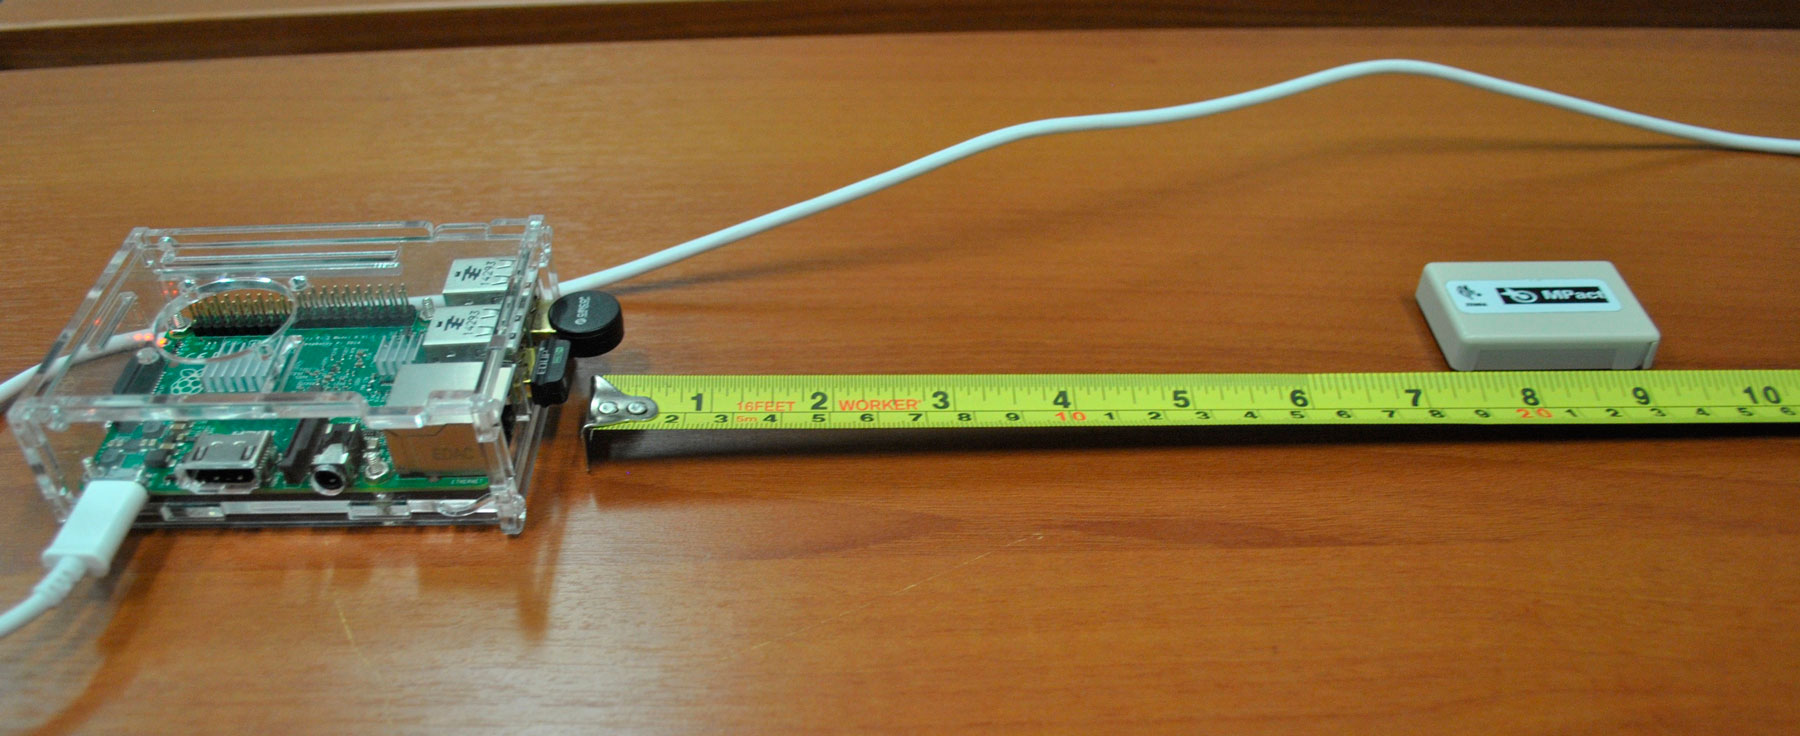
\includegraphics[width=0.8\textwidth]{img/ambiente2.jpg}
	\end{center}
	\legend{Fonte: elaborado pelo autor}
\end{figure}

Durante essa etapa não foram levados em consideração conexões com LEDs, botões e display LCD para a montagem do protótipo pois esses componentes foram definidos posteriormente. Os estudos e testes desses materiais foram realizados na segunda etapa, para que as escolhas fossem validadas.

% ----------------------------------------------------------
\section{Segunda Etapa - Planejamento do Protótipo}\label{sec:segunda-etapa}
% ----------------------------------------------------------

Para que o protótipo pudesse ser bem planejado, parâmetros foram definidos:

\begin{alineas}
	\item ter uma interface amigável e simples para interação com o software;
	\item ser bem apresentável, com cores marcantes e boa construção;
	\item mostrar informações relevantes sobre o sistema - aplicação, software e sistema (Linux e \textit{RPi});
	\item ser construído em um único pacote, não muito grande nem muito pequeno;
\end{alineas}

Seguindo esses parâmetros, a primeira busca foi por um recipiente para alocar todos os componentes necessários, de forma que tudo ficasse bem protegido. Para tal, escolheu-se uma caixa de metal, derivada de uma antiga caixa de cigarros, apresentado na \autoref{sec:acess-prototipo}.

O material foi cortado primeiramente na parte de baixo de forma que acomodasse o \textit{RPi} deixando todas as conexões disponíveis para futuro desenvolvimento e facilidade de acessar as portas. Foram realizados furos na parte do fundo para fixação do \textit{RPi} com parafusos, arruelas e porcas, conforme \autoref{fig:rpi-caixa}.

% TODO - FOTO DO FUNDO COM OS PARAFUSOS

\begin{figure}[htb]
	\caption{\label{fig:rpi-caixa}\textit{RPi} preso na caixa, com as portas acessíveis}
	\begin{center}
		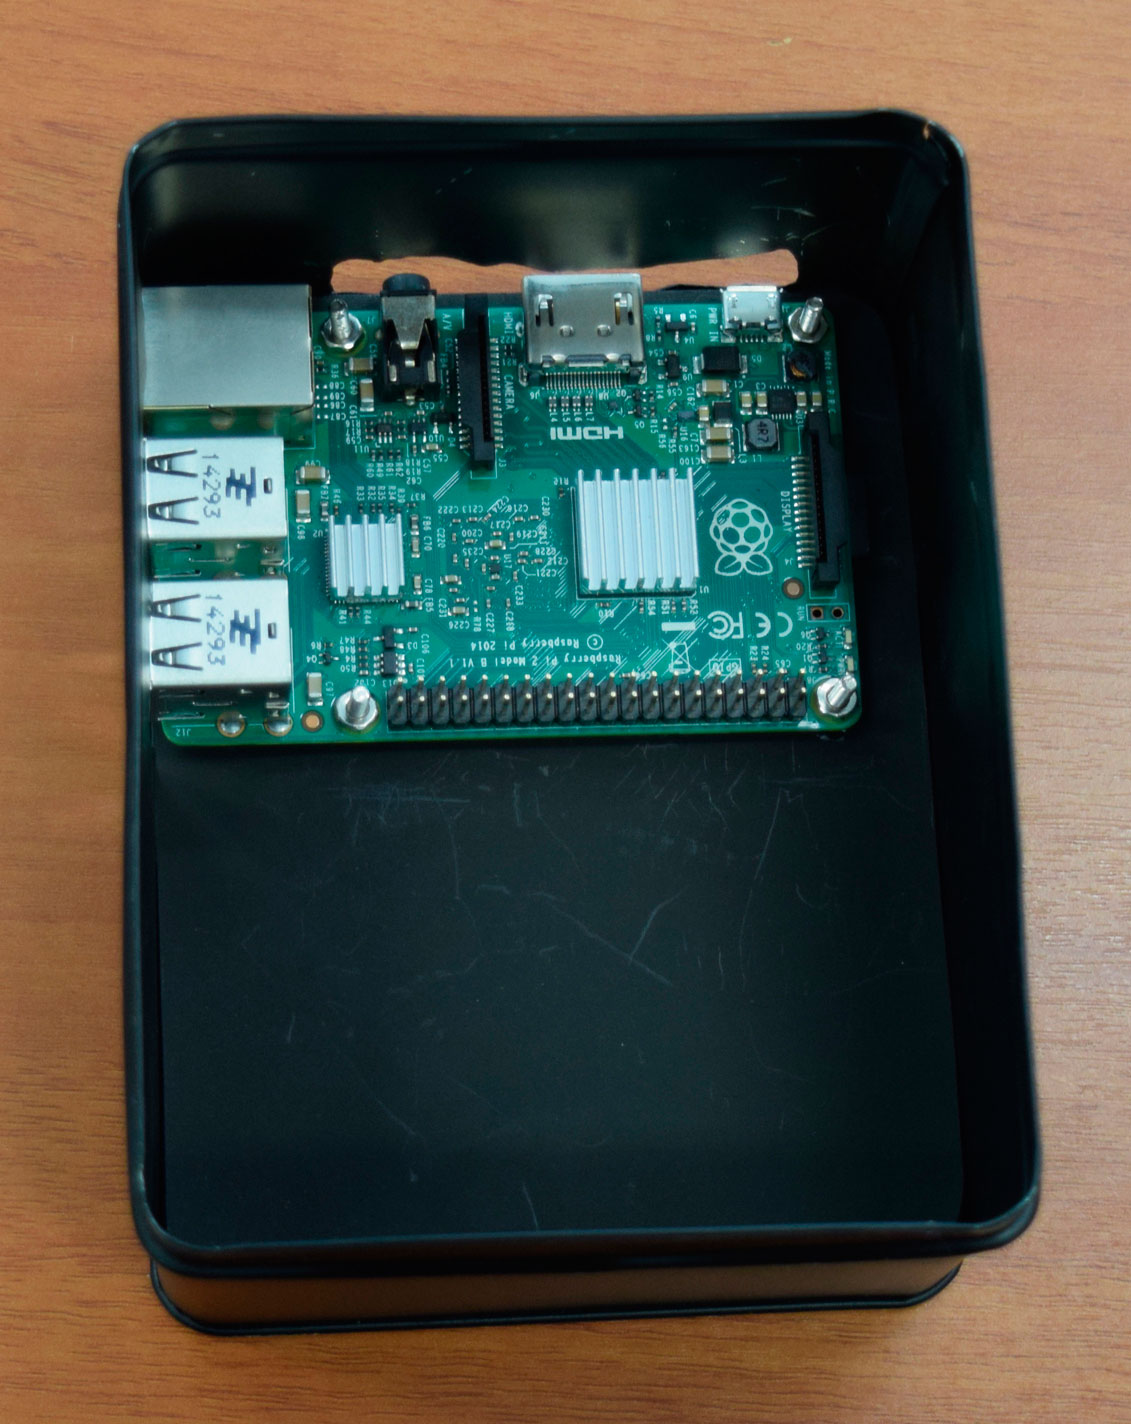
\includegraphics[width=0.6\textwidth]{img/rpi-caixa.jpg}
	\end{center}
	\legend{Fonte: elaborado pelo autor}
\end{figure}

Dessa maneira o RPi ficou bem preso na parte de baixo, liberando a tampa para instalação da interface com o usuário.

O próximo passo foi para definir a interface com o usuário. Para que os parâmetros fossem cumpridos, os seguintes itens necessários foram elencados:

\begin{alineas}
	\item apresentar informação em que consistia se o sistema está executando a aplicação corretamente - para tal definiu-se o uso de um LED verde;
	\item apresentar informação em que consistia se o sistema tem conexão com a internet - para tal definiu-se o uso de um LED amarelo;
	\item apresentar informação em que consistia se um \textit{beacon} está no alcance - para tal definiu-se o uso de um LED azul;
	\item apresentar várias informações textuais sobre o estado atual do sistema, assim como \textit{beacons} no alcance, histórico, dados do Linux, endereço de IP, temperatura da CPU - para tal, definiu-se o uso de um display LCD de 16 colunas por 2 linhas.
\end{alineas}

Como o display era pequeno e não apresentou todas as informações de uma só vez, decidiu-se pela utilização de navegação por páginas, de forma que as informações fossem alteradas conforme avançasse nas páginas. Para que a navegação fosse realizada de maneira agradável e apresentável, os seguintes itens foram escolhidos:

\begin{alineas}
	\item LEDs indicando qual página está - definiu-se pelo uso de três LEDs verde;
	\item botões do tipo clique para navegar a direita e esquerda nas páginas principais, e entre as páginas secundárias.
\end{alineas}

Com os componentes bem definidos, a interface foi concebida inicialmente em rascunhos no papel. Foi necessário realizar testes com os LEDs, display LCD e botões na protoboard de forma que todos esses componentes pudessem ser conectados ao mesmo tempo (\autoref{fig:proto-lcd} e \autoref{fig:proto-leds}). 

\begin{figure}[htb]
	\centering
 	\begin{minipage}{0.47\textwidth}
		\centering
		\caption{\label{fig:proto-lcd}Estudo de conexão e programação com display LCD}
		\includegraphics[width=1\textwidth]{img/proto-lcd.jpg}
		\legend{Fonte: elaborado pelo autor}
	\end{minipage}
	\hfill
	\begin{minipage}{0.47\textwidth}
		\centering
		\caption{\label{fig:proto-leds}Conexão com LEDs, display e botão na protoboard}
		\includegraphics[width=1\textwidth]{img/proto-leds.jpg}
		\legend{Fonte: elaborado pelo autor}
	\end{minipage}
\end{figure}

Nesse momento definiu-se o uso de Node.js (detalhado na \autoref{sec:node-js}) para o desenvolvimento, pois foram encontrados diversos tutoriais\footnote{\url{http://thejackalofjavascript.com/rpi-16x2-lcd-print-stuff/}}\footnote{\url{http://odesenvolvedor.andafter.org/publicacoes/controlando-gpio-do-raspberrypi-com-nodejs.html}}\footnote{\url{https://learn.adafruit.com/node-embedded-development/why-node-dot-js}} e bibliotecas\footnote{\url{https://www.npmjs.com/package/lcd}}\footnote{\url{https://www.npmjs.com/package/onoff}} que facilitaram a conexão com todos os componentes.

Após realizar todos os estudos e testes de conexão com sucesso, o próximo passo foi a montagem da interface na caixa de metal. Primeiro os cortes foram feitos com uma ferramenta específica tipo esmeril, em seguida a caixa foi pintada com tinta preta fosca (\autoref{fig:pintar-1} e \autoref{fig:pintar-2}) para que o protótipo ficasse com boa construção e visualização.

Foram necessários soldas e montagem dos outros componentes em placas para que tudo ficasse organizado e fácil de ser trocado, caso necessário. As conexões das GPIOs com os componentes de hardware estão marcados na \autoref{fig:pinout-gpio}.

\begin{figure}[htb]
	\centering
 	\begin{minipage}{0.45\textwidth}
		\centering
		\caption{\label{fig:pintar-1}Pintura da caixa de metal - tampa}
		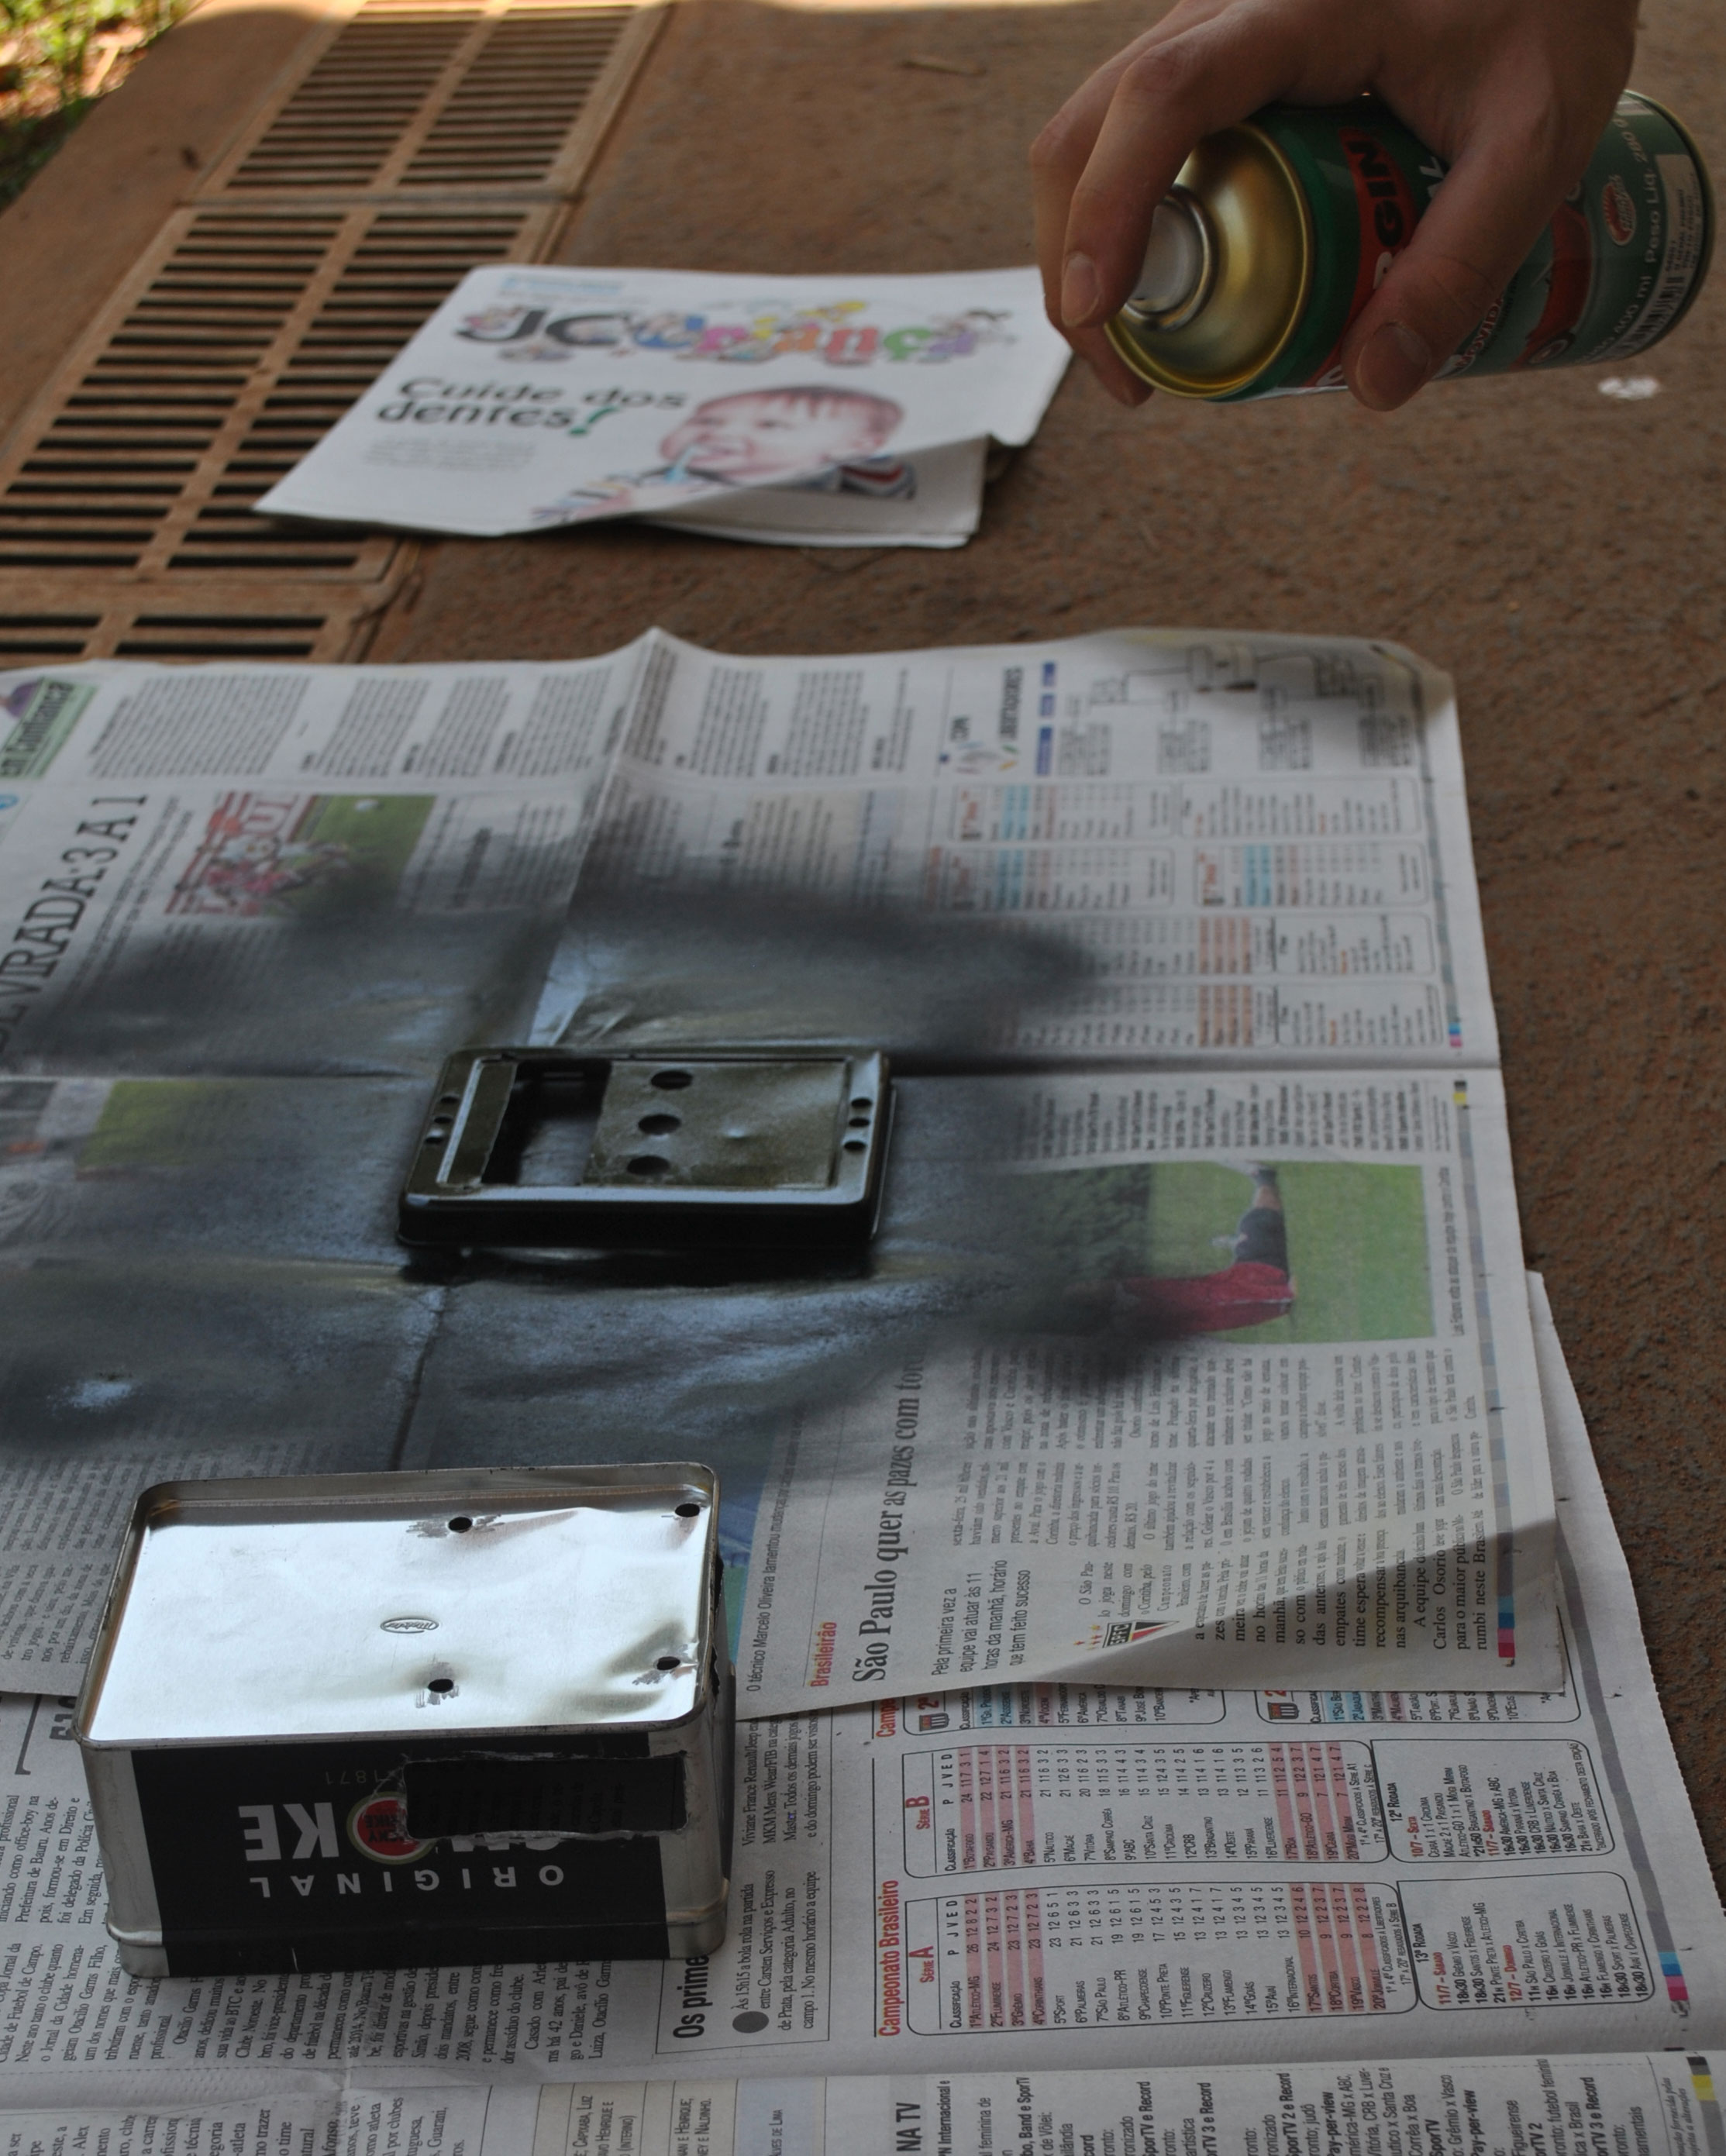
\includegraphics[width=1\textwidth]{img/pintar-1.jpg}
		\legend{Fonte: elaborado pelo autor}
	\end{minipage}
	\hfill
	\begin{minipage}{0.45\textwidth}
		\centering
		\caption{\label{fig:pintar-2}Pintura da caixa de metal - base}
		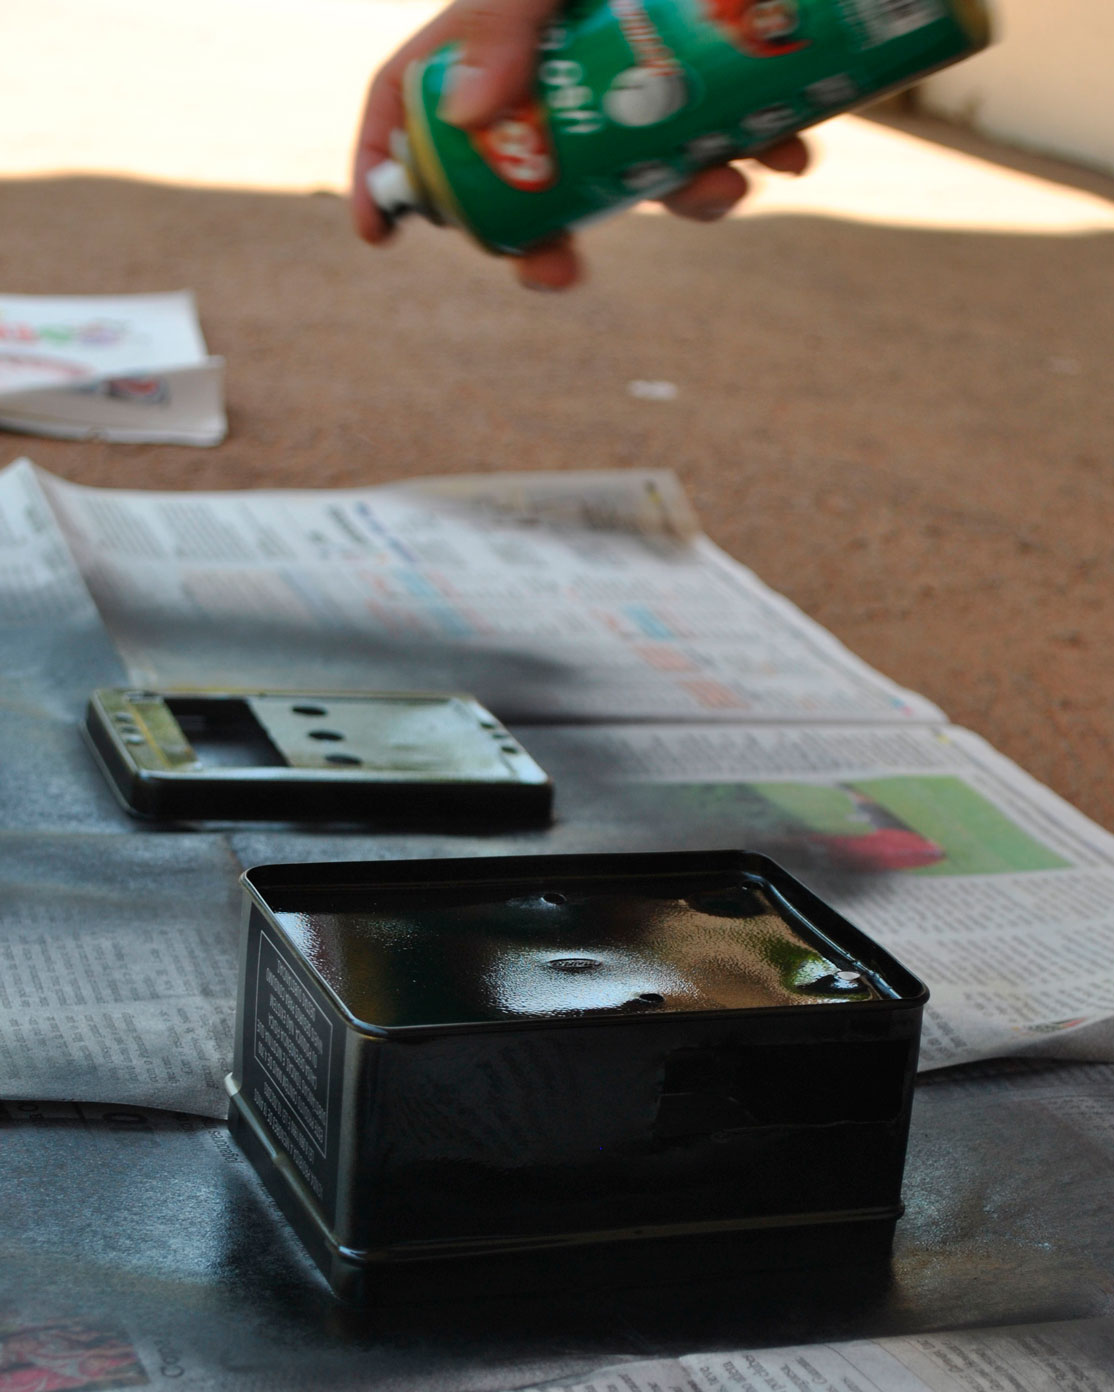
\includegraphics[width=1\textwidth]{img/pintar-2.jpg}
		\legend{Fonte: elaborado pelo autor}
	\end{minipage}
\end{figure}

Cada LED foi conectado a uma GPIO, a um resistor de 330$\Omega$, e ao GND. Os botões foram conectados seguindo o modelo da \autoref{fig:push-btn-sketch}. O display foi conectado diretamente a cada GPIO marcada, e também ao +5V e GND para alimentação. 

O modelo de display LCD utilizado também tem um pino que utiliza voltagem variável para iluminar cada caractere (contraste de cada letra), e um pino para a iluminação do fundo (azul). Para essas conexões foram utilizados potenciômetros de 10K, para facilitar mudanças caso necessário (\autoref{fig:potentiometer}). Dessa forma, só é necessário girar o pino do potenciômetro para alterar a saída.

\begin{figure}[htb]
	\centering
 	\begin{minipage}{0.45\textwidth}
		\centering
		\caption{\label{fig:push-btn-sketch}Modelo de conexão dos botões}
		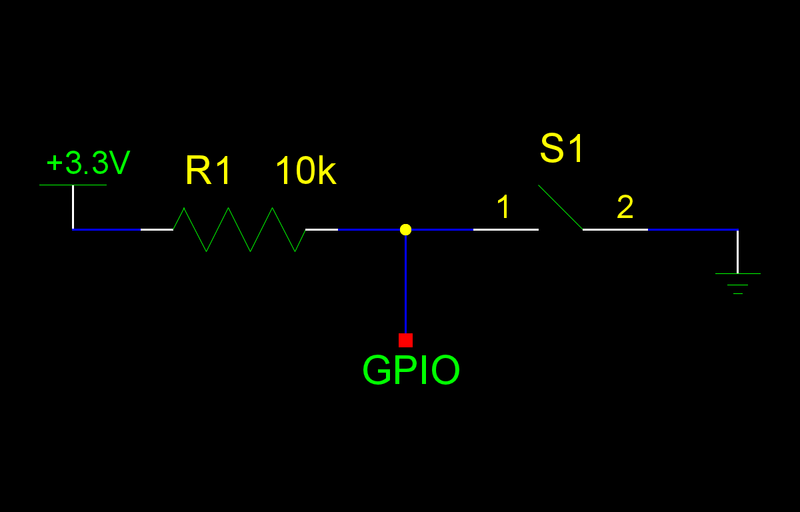
\includegraphics[width=1\textwidth]{img/push-btn-sketch.png}
		\legend{Fonte: \cite{push-button}}
	\end{minipage}
	\hfill
	\begin{minipage}{0.45\textwidth}
		\centering
		\caption{\label{fig:potentiometer}Potenciômetros de configuração do display LCD}
		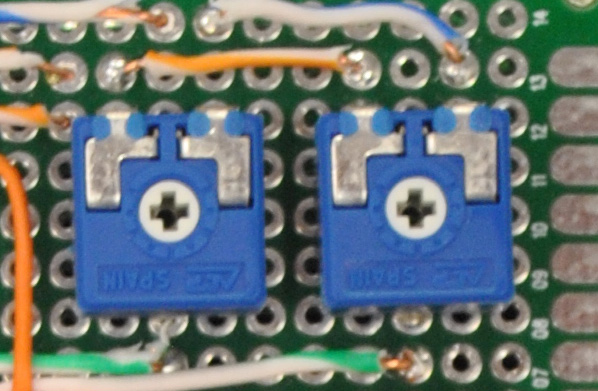
\includegraphics[width=1\textwidth]{img/potentiometer.jpg}
		\legend{Fonte: elaborado pelo autor}
	\end{minipage}
\end{figure}

\begin{figure}[htb]
	\caption{\label{fig:pinout-gpio}Circuito de conexão das GPIOs}
	\begin{center}
		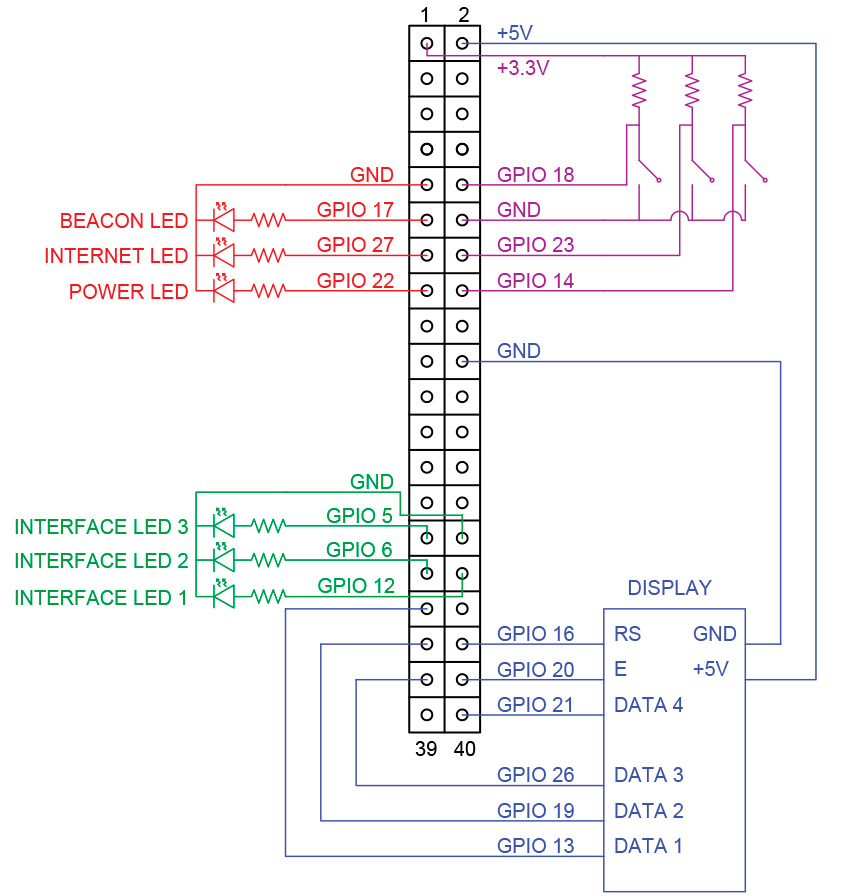
\includegraphics[width=0.8\textwidth]{img/pinout-gpio.jpg}
	\end{center}
	\legend{Fonte: elaborado pelo autor}
\end{figure}

Foram utilizados seis GPIOs para os LEDs, três para os botões e seis para o display, totalizando 15 GPIOs de 17 disponíveis. As GPIOs utilizadas foram:

\begin{alineas}
	\item Para os LEDs de interface (topo), GPIO 12, 6 e 5, respectivamente 1, 2 e 3;
	\item Para os LEDs de informação (baixo), GPIO 22, 27 e 17, respectivamente Power, Internet e Beacon;
	\item Para os botões, GPIOs 24, 23 e 18, respectivamente botão esquerdo, central e direito;
	\item Para o display de LCD, GPIOs 16, 20, 13, 19, 26, 21, respectivamente Register Select, Enable, Data 1, Data 2, Data 3 e Data 4.
	\nota{Os números das GPIOs foram escolhidos devido a proximidade e agrupamento dos componentes.}
\end{alineas}

De forma que a tampa saísse facilmente optou-se por usar um cabo flat frequentemente usado em HDs antigos (padrão IDE) conectado ao \textit{RPi} e a uma placa central com duas fileiras de 20 pinos.

Utilizando os fios internos de cabo de rede para conexão entre os componentes nas placas, o mesmo cabo flat cortado para conexão entre as placas para uma maior flexibilidade e facilidade de mudanças, criou-se o controle da interface, como pode ser visto na \autoref{fig:interface-traz1} e \autoref{fig:interface-traz2}.

\begin{figure}[htb]
	\centering
 	\begin{minipage}{0.45\textwidth}
		\centering
		\caption{\label{fig:interface-traz1}Parte interna da interface - parcialmente desmontada}
		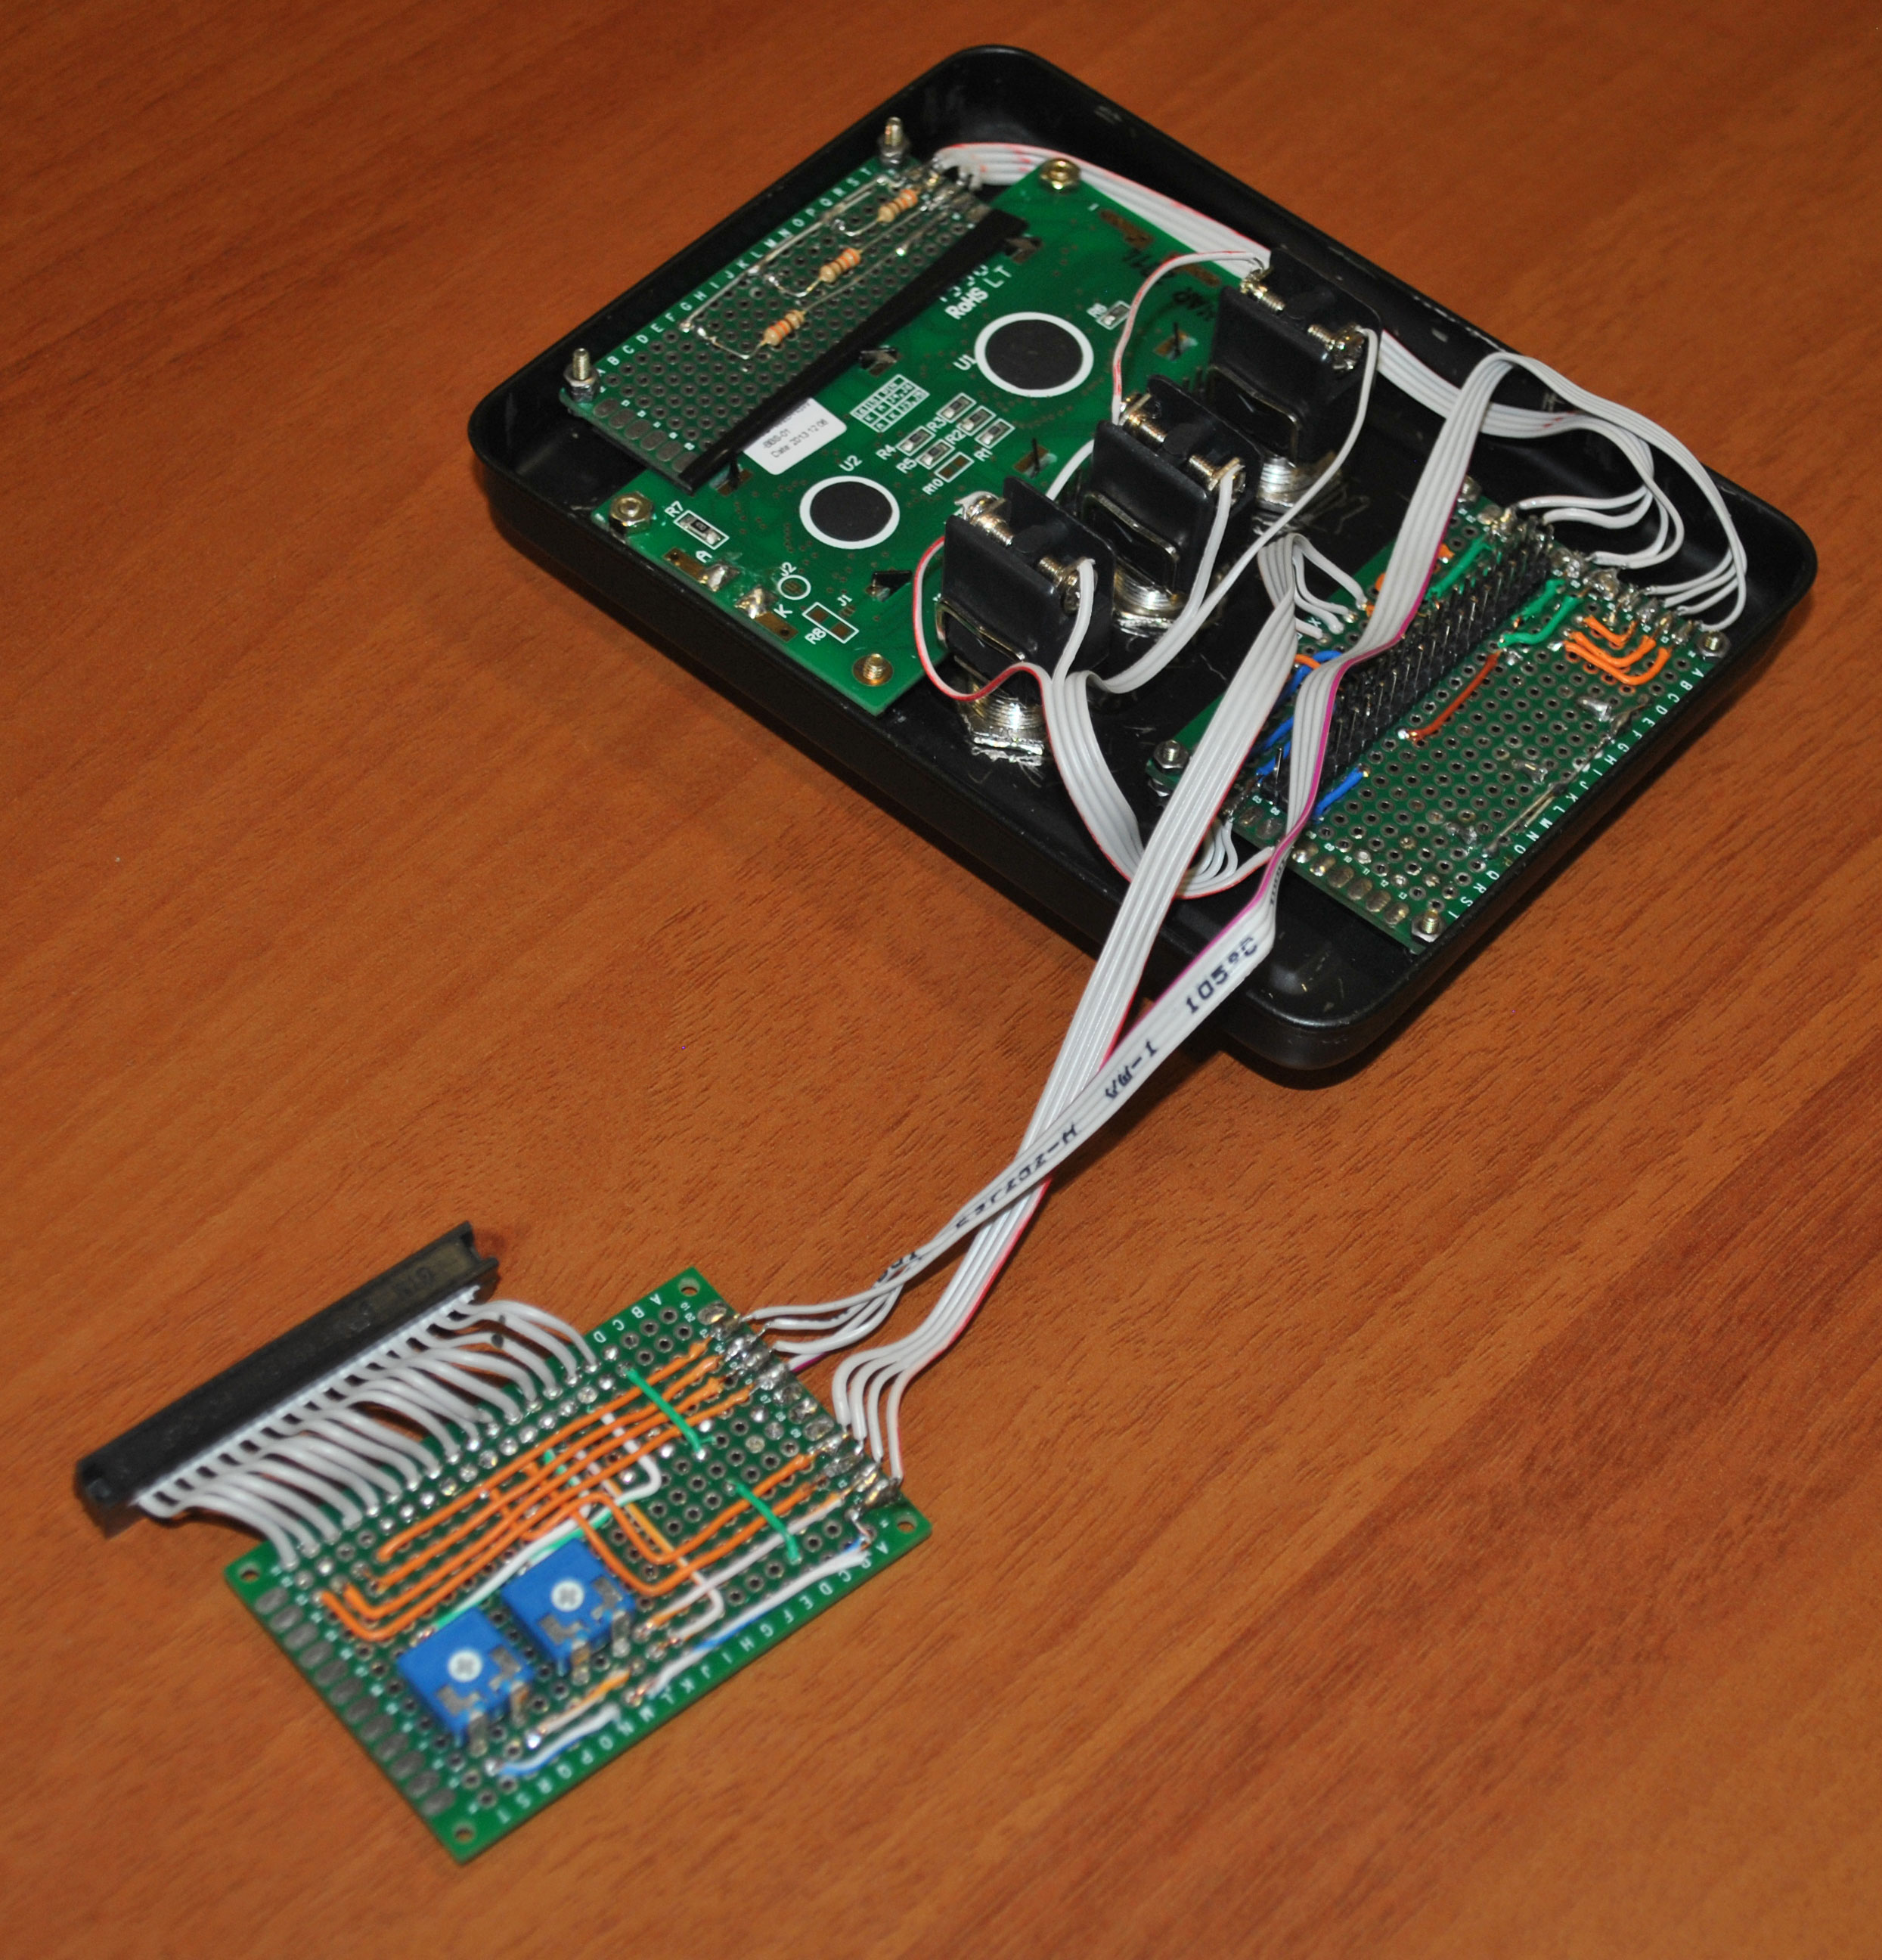
\includegraphics[width=1\textwidth]{img/interface-traz1.jpg}
		\legend{Fonte: elaborado pelo autor}
	\end{minipage}
	\hfill
	\begin{minipage}{0.45\textwidth}
		\centering
		\caption{\label{fig:interface-traz2}Parte interna da interface - completamente montada}
		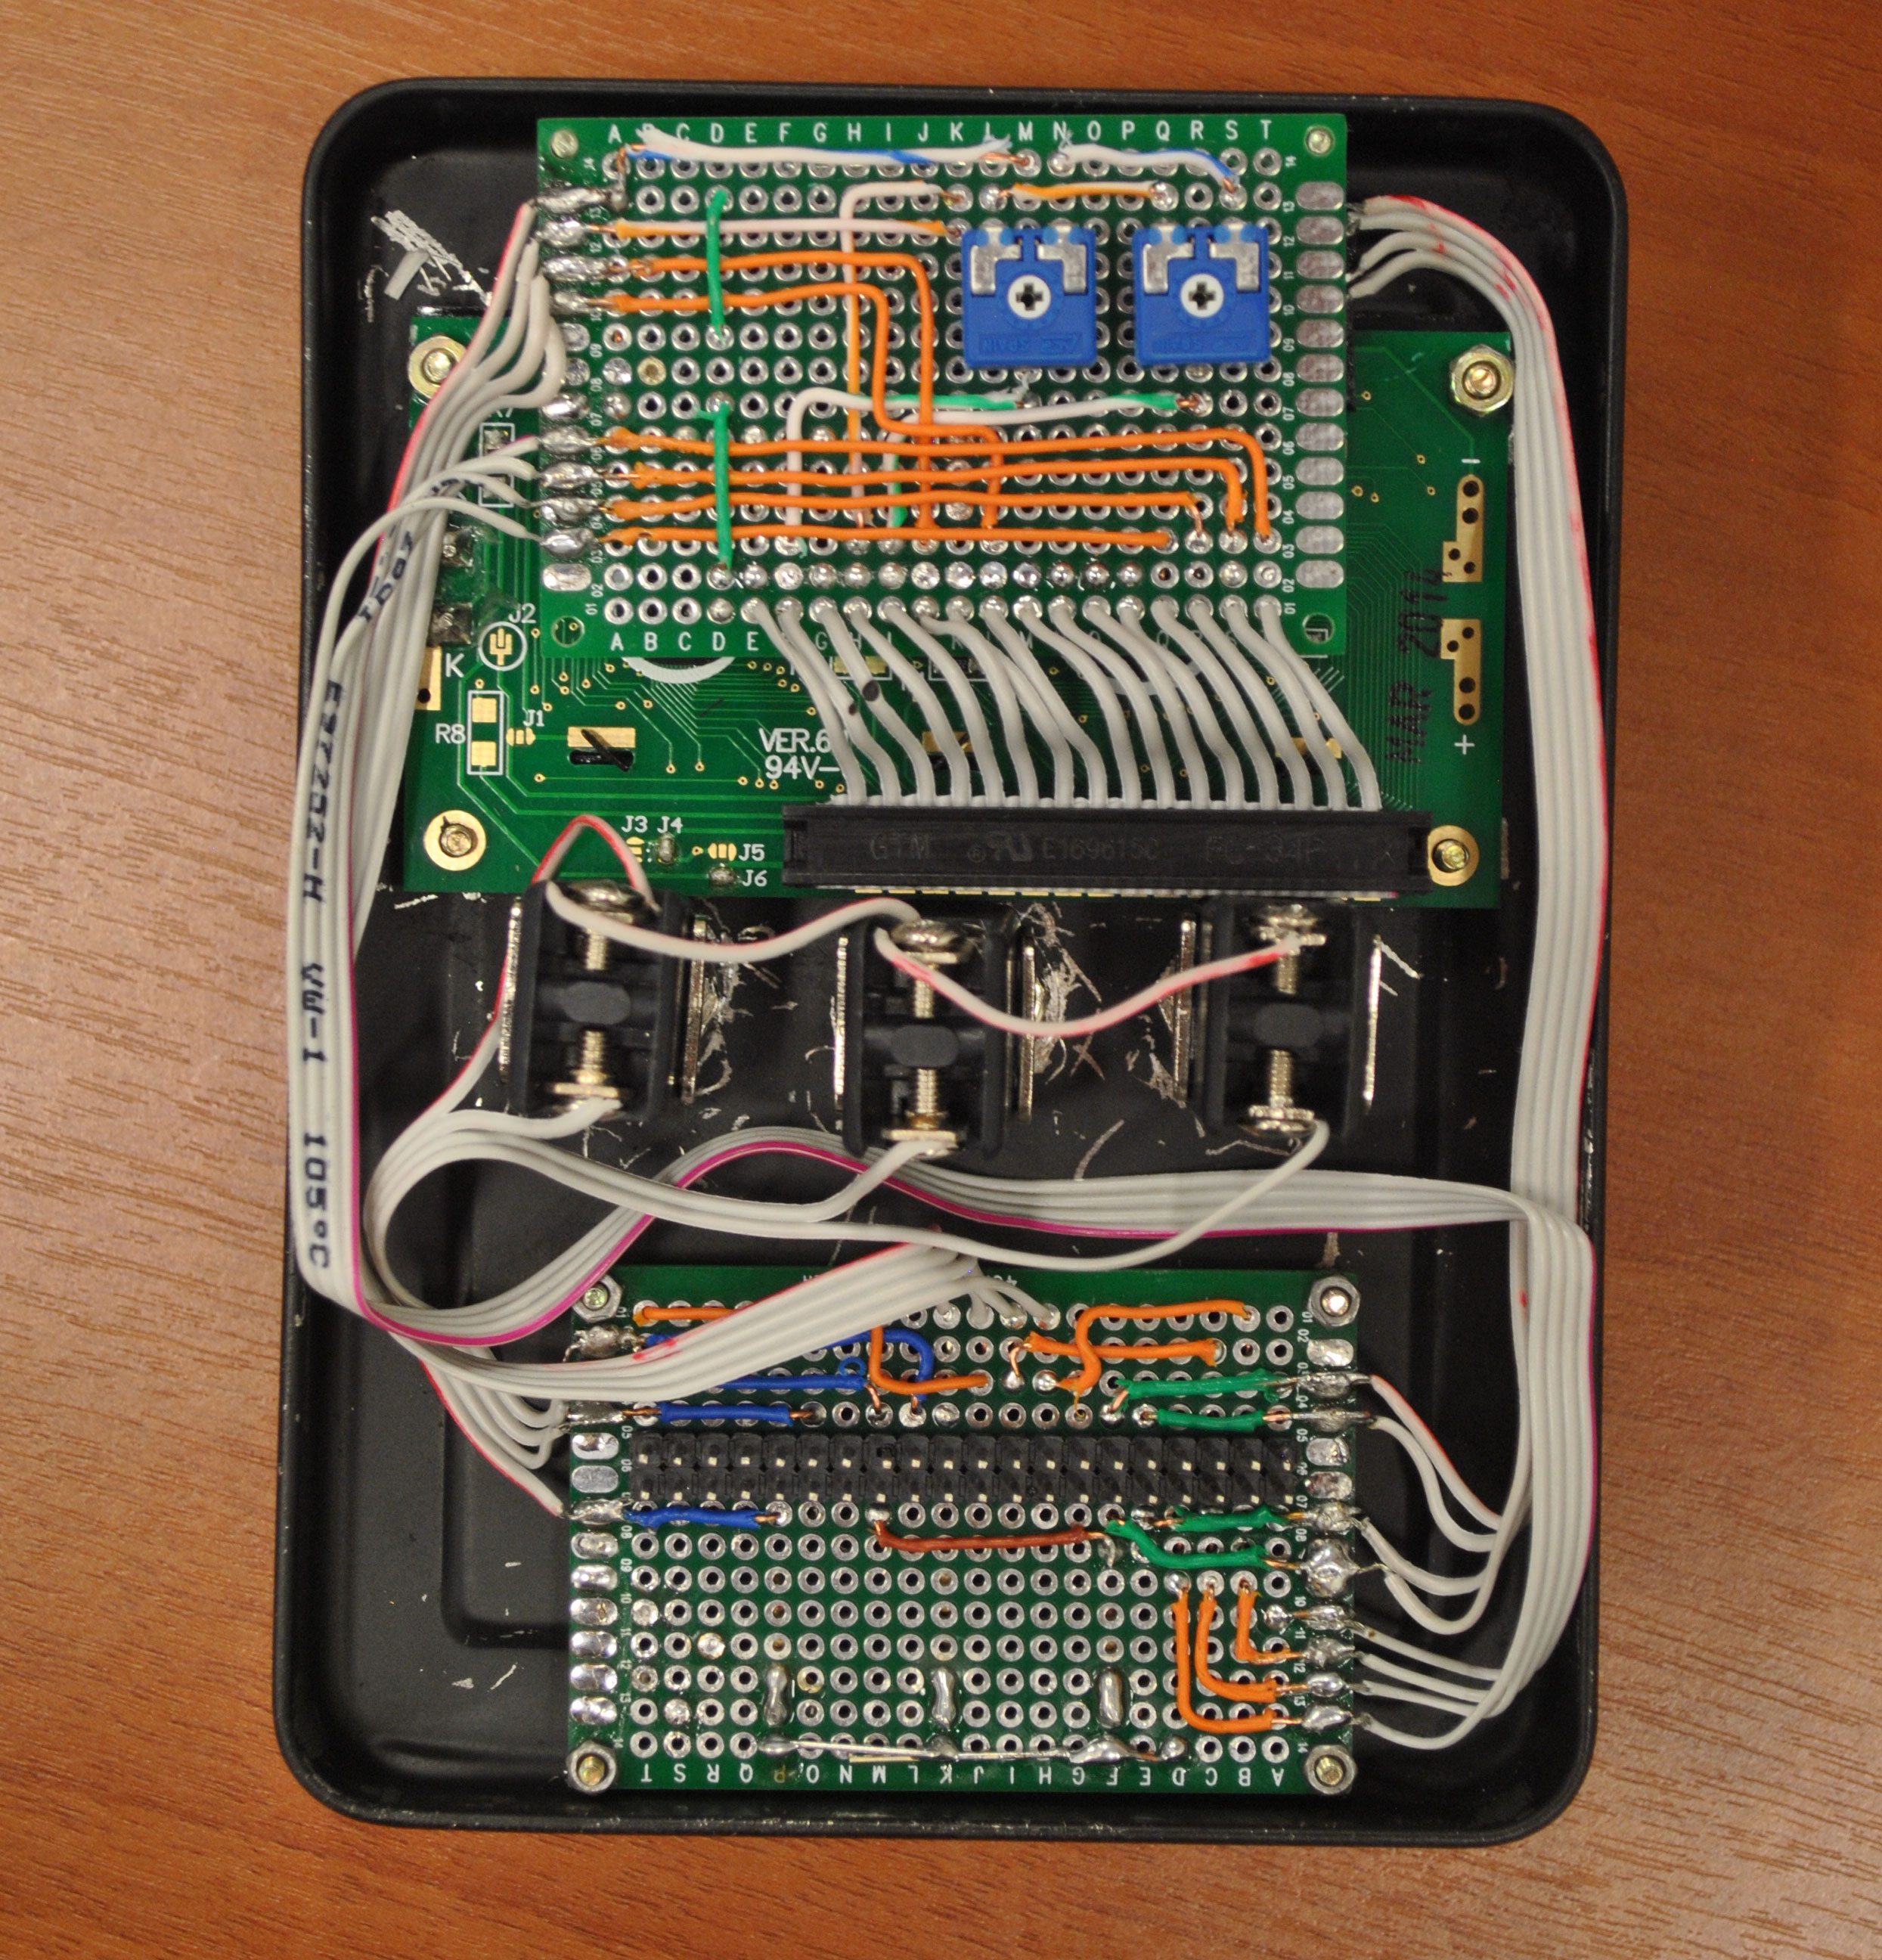
\includegraphics[width=1\textwidth]{img/interface-traz2.jpg}
		\legend{Fonte: elaborado pelo autor}
	\end{minipage}
\end{figure}

As placas internas da interface foram afixadas com cola quente, para que os cabos fossem reforçados e nenhuma conexão fosse quebrada. Tampa e base foram conectados com o cabo flat (\autoref{fig:tampa-base}) e o protótipo ficou pronto para desenvolvimento da aplicação.

\begin{figure}[htb]
	\centering
 	\begin{minipage}{0.45\textwidth}
		\centering
		\caption{\label{fig:tampa-base}Conexão da tampa com a base}
		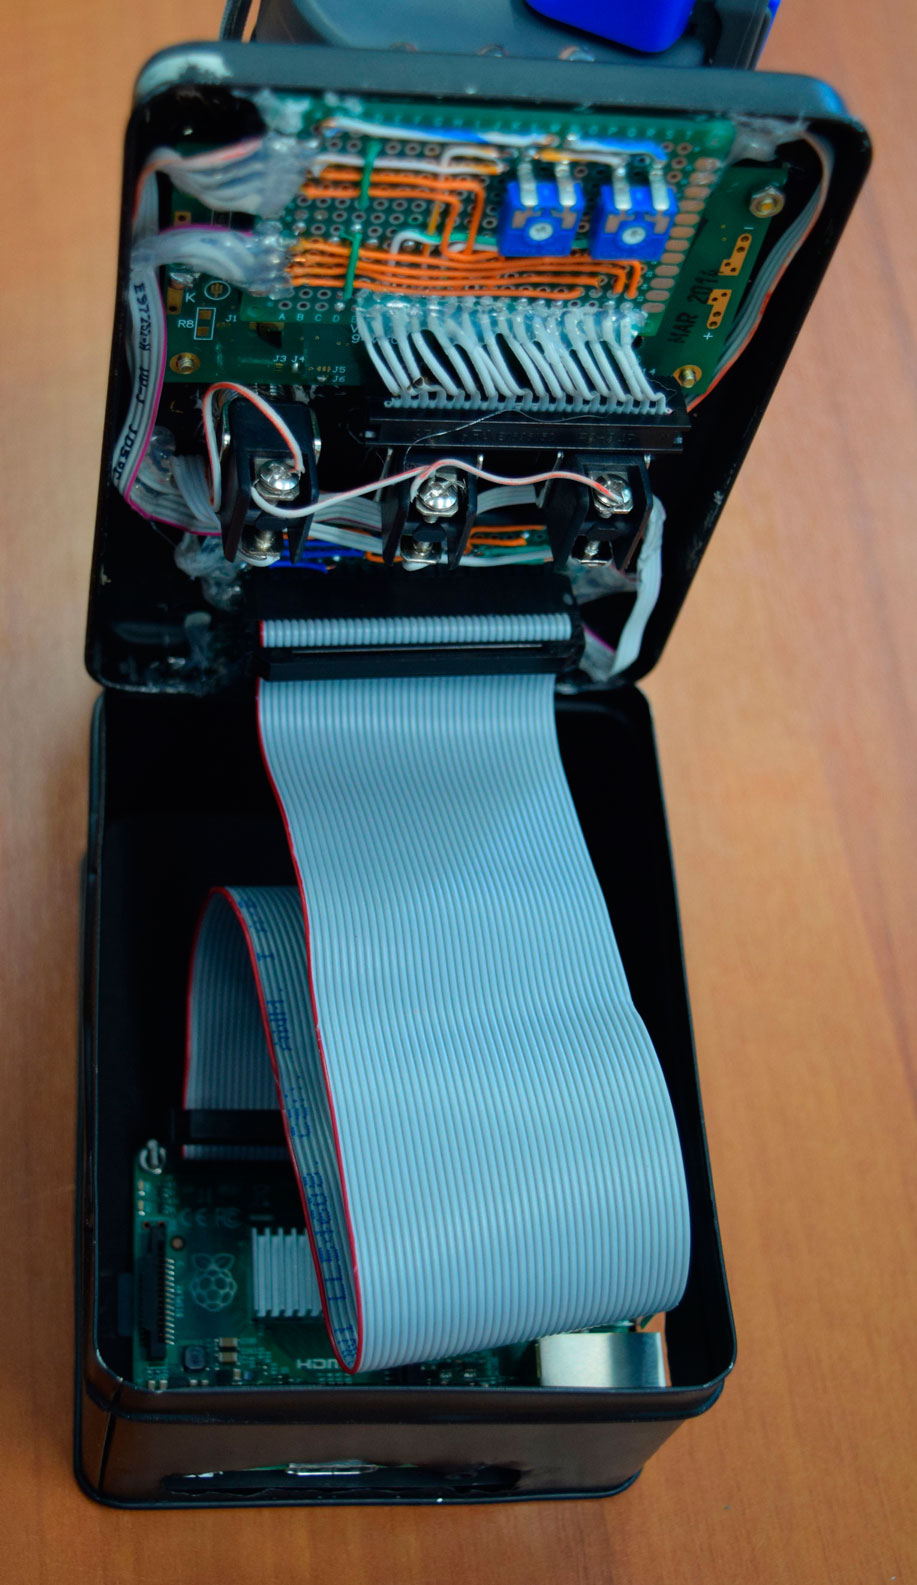
\includegraphics[width=0.84\textwidth]{img/tampa-base.jpg}
		\legend{Fonte: elaborado pelo autor}
	\end{minipage}
	\hfill
	\begin{minipage}{0.45\textwidth}
		\centering
		\caption{\label{fig:prot-final}Criação e montagem do protótipo finalizada}
		\includegraphics[width=1\textwidth]{img/prot-final-2.jpg}
		\legend{Fonte: elaborado pelo autor}
	\end{minipage}
\end{figure}

Após o hardware estar totalmente montado, as informações apresentadas nas telas foram elaboradas:

\begin{alineas}
	\item A primeira tela mostra informações sobre os \textit{beacons} no alcance, ou caso não haja nenhum, apresenta o texto "\textit{Aguardando beacons}". As subtelas apresentam informações sobre quais \textit{beacons} estão no alcance, sendo o nome atribuidos a eles ou então o texto "\textit{Desconhecido}"\ caso não esteja no banco de dados. A quantidade de subtelas depende da quantidade de \textit{beacons} no alcance, por isso não se sabe ao certo a quantidade total;
	\item A segunda tela apresenta um histórico dos \textit{beacons} encontrados durante a execução do programa, com um contador da quantidade de \textit{beacons} no histórico, e as subtelas apresentam o nome do \textit{beacon} encontrado em ordem numérica. Se um \textit{beacon} for encontrado diversas vezes, será repetido nas subtelas. Conforme a primeira tela, a quantidade de subtelas depende da quantidade de \textit{beacons} no histórico, por isso não se sabe ao certo a quantidade total;
	\item A terceira tela apresenta informações relevantes sobre o sistema, sendo elas:
	\begin{subalineas}
		\item Primeira subtela apresenta o \textit{load average}\footnote{Segundo \citeonline{load-average}, essa informação de três números apresenta a média de carga da CPU por um certo tempo. O primeiro número é a média no último minuto, o segundo número é a média nos últimos cinco minutos, e o terceiro número é a média nos últimos quinze minutos} do sistema Linux. É relevante para saber se o sistema está muito carregado ou trabalhando tranquilamente;
		\item Segunda subtela apresenta a temperatura do processador. É relevante para saber se o sistema está trabalhando a uma temperatura segura ou está sobreaquecendo;
		\item Terceira subtela apresenta o endereço de IP privado da rede. É de extrema importância para conexão remota, pois é esse endereço que é utilizado para conexão via \textit{SSH};
		\item Quarta subtela apresenta o endereço de IP público da rede. É relevante para saber se está conectado direto a internet (o IP privado será igual ao IP público) ou em uma subrede, como de uma residência ou do laboratório.
	\end{subalineas}
\end{alineas}

Após todos esses passos o protótipo estava bem definido para o desenvolvimento.

% ---
\subsection{Logotipo e Nome para o Protótipo}\label{sec:logotipo-prototipo}
% ---

Por ser um produto, decidiu-se que o protótipo deveria ter um nome e logotipo. Durante algumas reuniões de \textit{brainstorm}, o nome \textit{Peacon} surgiu e foi o escolhido. Esse nome deriva das palavras \textit{Pi}  + \textit{beacon}.

Juntando todos os atributos do Peacon, criou-se um logotipo que identificasse muito bem todas as funcionalidades do protótipo (\autoref{fig:logo-peacon}). Adesivos foram criados para colar no protótipo e identificar o produto. Também foi criado um logotipo menor, para colar em componentes secundários (\autoref{fig:logo-menor-peacon}).


\begin{figure}[htb]
	\centering
 	\begin{minipage}{0.45\textwidth}
		\centering
		\caption{\label{fig:logo-peacon}Logotipo criado para o protótipo}
		
\includegraphics[width=1\textwidth]{img/logo-peacon.png}
		\legend{Fonte: elaborado pelo autor}
	\end{minipage}
	\hfill
	\begin{minipage}{0.45\textwidth}
		\centering
		\caption{\label{fig:logo-menor-peacon}Logotipo menor criado para o protótipo}
		
\includegraphics[width=1\textwidth]{img/logo-menor-peacon.png}
		\legend{Fonte: elaborado pelo autor}
	\end{minipage}
\end{figure}


% ---
\subsection{Problemas Enfrentados}\label{sec:problemas-enfrentados}
% ---

Durante os estudos e testes dos LEDs na protoboard utilizou-se resistores de 330$\Omega$ para conexão correta. Quanto maior o valor da resistência, menor brilho o LED apresenta. Como os componentes estavam na protoboard, não percebeu-se que os LEDs utilizados eram de alto brilho.

Para soldagem final dos componentes, preferiu-se por manter os resistores de 330$\Omega$ por questões práticas. Porém os LEDs ficaram com muito brilho, incomodando qualquer pessoa que olhasse diretamente para o protótipo, conforme \autoref{fig:led-forte-1} e \autoref{fig:led-forte-2}.

Como os componentes já estavam afixados com cola quente, substituir os resistores levaria muito tempo e possivelmente atrasaria o desenvolvimento do projeto, portanto optou-se por manter dessa maneira. Para um futuro protótipo, resistores maiores, ou LEDs com menos brilho podem ser utilizados.

\begin{figure}[htb]
	\centering
 	\begin{minipage}{0.45\textwidth}
		\centering
		\caption{\label{fig:led-forte-1}LED de alto brilho ao olhar diretamente}
		\includegraphics[width=1\textwidth]{img/led-forte-1.jpg}
		\legend{Fonte: elaborado pelo autor}
	\end{minipage}
	\hfill
	\begin{minipage}{0.45\textwidth}
		\centering
		\caption{\label{fig:led-forte-2}LEDs de alto brilho refletindo na mesa}
		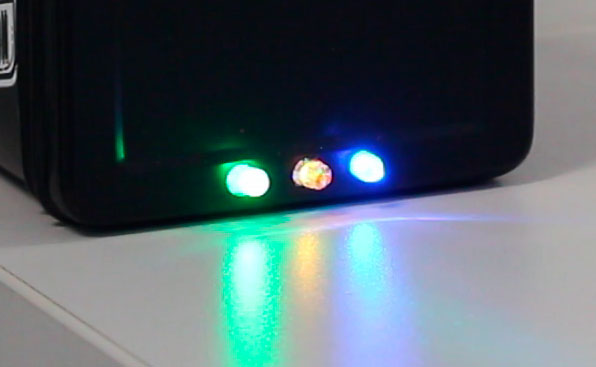
\includegraphics[width=1\textwidth]{img/led-forte-2.jpg}
		\legend{Fonte: elaborado pelo autor}
	\end{minipage}
\end{figure}

% ----------------------------------------------------------
\section{Terceira Etapa - Desenvolvimento e Testes da Aplicação}\label{sec:terceira-etapa}
% ----------------------------------------------------------

A aplicação foi dividida em módulos por maior facilidade de desenvolvimento, testes e descoberta de erros. Um arquivo de configurações globais, nomeado \textit{globals-config.js}, foi utilizado para todas as definições de constantes de forma a facilitar futuras mudanças, caso necessário. 

% ---
\subsection{Primeiro Módulo - Biblioteca Auxiliar}\label{sec:primeiro-modulo}
% ---

O primeiro módulo desenvolvido foi a interface, que consiste da conexão com LEDs, botões e display LCD. Optou-se por criar uma biblioteca auxiliar para abstrair métodos repetitivos e também irrelevantes para os outros módulos. Como esse módulo é o meio de acesso do código principal aos componentes de hardware, foram adicionados trechos de teste para acender o LED e apagar o LED pela linha de comando, de forma que os testes de funcionalidade pudessem ser realizados.

Durante a fase de testes do primeiro módulo, um fato interessante ocorreu. Ao clicar uma única vez em um botão, em algumas vezes o código executava dois, três ou até mais cliques de botão. Pesquisando mais a fundo sobre esse erro, uma informação nova surgiu. 

Botões mecânicos não criam ou perdem o contato corretamente, conforme caso ideal e perfeito representado no gráfico apresentado na \autoref{fig:debounce-graph-1}. Em vez disso, podem oscilar rapidamente no momento do clique ou ao soltar o botão, conforme gráfico apresentado na \autoref{fig:debounce-graph-2}. \cite{debounce-graph}. Esse efeito é conhecido como \textit{bounce}, ou ruído.

\begin{figure}[htb]
	\centering
 	\begin{minipage}{0.45\textwidth}
		\centering
		\caption{\label{fig:debounce-graph-1}Gráfico ideal de um clique de botão}
		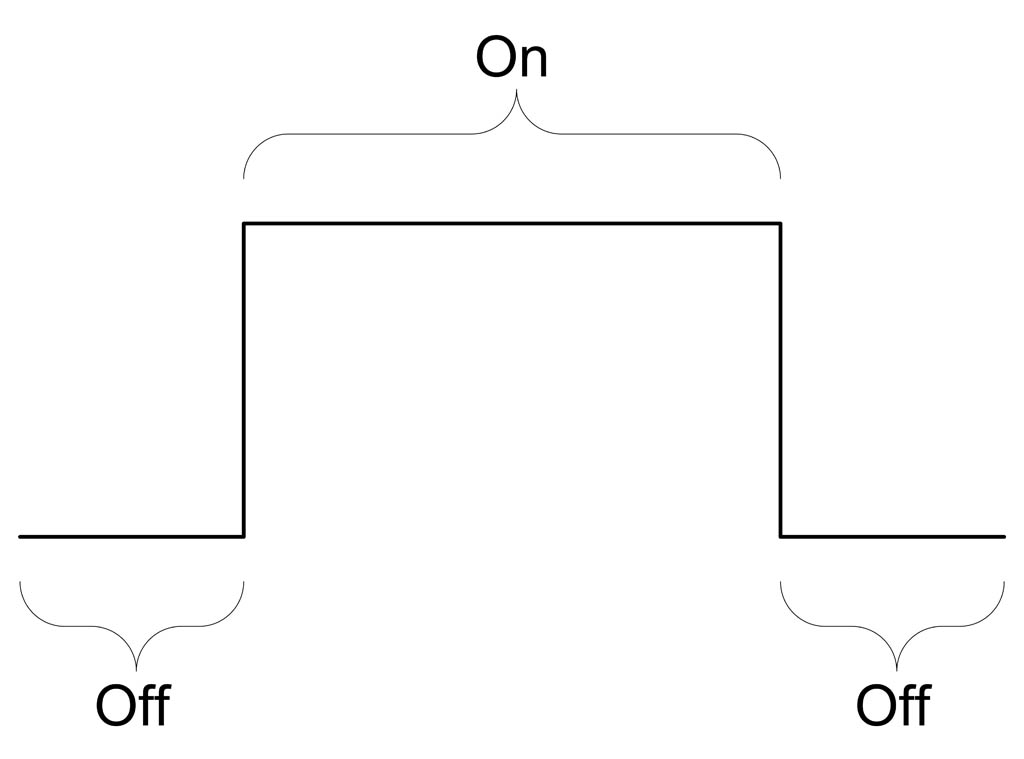
\includegraphics[width=0.8\textwidth]{img/debounce-graph-1.jpg}
		\legend{Fonte: \cite{debounce-graph}}
	\end{minipage}
	\hfill
	\begin{minipage}{0.45\textwidth}
		\centering
		\caption{\label{fig:debounce-graph-2}Gráfico real de um clique de botão}
		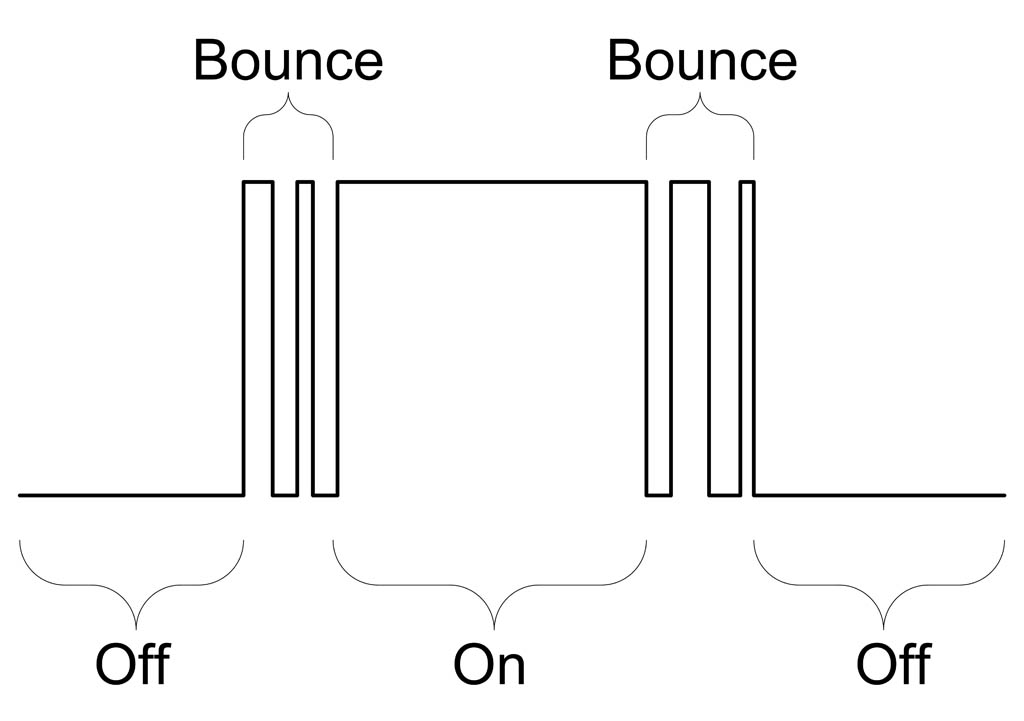
\includegraphics[width=0.8\textwidth]{img/debounce-graph-2.jpg}
		\legend{Fonte: \cite{debounce-graph}}
	\end{minipage}
\end{figure}

A solução para resolver esse problema (denominada \textit{debounce}) foi de bloquear todos os cliques após o primeiro clique via programação por determinado tempo (em milissegundos), de forma que não interferisse diretamente nos cliques reais do usuário. Esse tempo foi determinado por testes repetitivos e por diferentes usuários em 200ms. Esse valor foi considerado ideal por evitar o ruído e não interferir em cliques seguidos do usuário. Valores maiores, como 300ms afetaram o clique do usuário, e valores inferiores como 100ms não evitaram totalmente o ruído.

% ---
\subsection{Segundo Módulo - Páginas e Navegação}\label{sec:segundo-modulo}
% ---

O segundo módulo consistiu da criação e navegação entre páginas. Para que as páginas secundárias pudessem ser dinamicamente inseridas nas telas, utilizou-se uma matriz de funções para lidar com a troca de informações na interface. 

Esse método foi muito eficaz e adaptou-se muito bem na metodologia de desenvolvimento para Node.js. O ato de mudar a tela executa a função na próxima posição do vetor. Isso permite que cada tela, com as suas particularidades, seja de fácil criação e alteração, incluindo-se ou retirando-se páginas primárias e secundárias.

Nos testes desse módúlo não surgiram problemas, erros ou \textit{bugs}, pela sua simplicidade de desenvolvimento. Nos próximos métodos, trechos criados nesse passo sofreram apenas pequenas alterações de adaptação.

% ---
\subsection{Terceiro Módulo - Identificação dos \textit{Beacons}}\label{sec:terceiro-modulo}
% ---

Nesse módulo foram implementadas as funções de identificação dos \textit{beacons}. Quando um \textit{beacon} entra no alcance, é salvo em um vetor auxiliar. 

Como os \textit{beacons} transmitem pacotes de tempos em tempos, houve necessidade de criar uma lógica para verificar se ainda estavam no alcance depois de determinado tempo. Para isso, no momento em que um pacote \textit{beacon} é identificado, dispara um evento a ser executado após um determinado tempo (em segundos). O valor do tempo de espera foi descoberto por meio de seguidos testes, e o valor ideal encontrado foi de 3 segundos.

O próximo passo foi apresentar nas páginas principais e secundárias a quantidade de \textit{beacons} descobertos, e implementar o histórico da aplicação. Nesse módulo os \textit{beacons} descobertos ainda não são salvos, permanecendo somente durante a execução do programa.

% ---
\subsubsection{Problemas Enfrentados}\label{sec:problema-quarto-modulo}
% ---

O módulo de identificação dos \textit{beacons} apresentou um problema constante em todas as primeiras execuções após reinicialização do \textit{RPi}. O módulo bluetooth não reportava nenhum pacote \textit{beacon}, e nenhuma descoberta era possível. 

Ao analisar a fundo esse problema, percebeu-se que o \textit{driver} desse módulo estava defeituoso, e nada poderia ser feito. A solução encontrada foi de reiniciar a interface bluetooth toda vez que o software fosse executado. Com essa solução, os pacotes \textit{beacon} apareceram e o software funcionava normalmente.

Após algumas semanas, ao avançar no desenvolvimento e testes, percebeu-se que o problema se agravou. Em alguns momentos aleatórios durante a execução do programa o módulo parava de funcionar totalmente, sendo necessária a reinicialização da interface.

Essa solução resolvia o problema momentaneamente. Não foram encontrados outros drivers ou solução para o problema, porém como não afetou o desenvolvimento e testes do protótipo não foi necessário a troca do módulo \textit{bluetooth}.

% ---
\subsection{Quarto Módulo - Busca no Banco de Dados}\label{sec:quarto-modulo}
% ---

Até o momento o software somente apresentava a quantidade de \textit{beacons} no alcance, e não identificava os mesmos. Nesse módulo foi implementado a busca no banco de dados pelas informações do \textit{beacon} para possível identificação.

O CouchDB tem uma busca muito fácil e prática por identificadores de documento. Para aproveitar essa funcionalidade, um padrão de identificadores e documentos foi criado:

\begin{verbatim}
Documento JSON para beacons conhecidos
[{
    "_id": "UUID-Major-Minor",
    "uuid": "numero-uuid",
    "major": "numero-major",
    "minor": "numero-minor",
    "name": "nome-beacon"
}]
\end{verbatim}

O campo \textit{\_id} é formado do número UUID, seguido pelo número \textit{Major}, e finalizado pelo número \textit{Minor}, todos separados pelo caractere - (menos). Exemplo de documento:

\begin{verbatim}
Exemplo de documento JSON para beacons conhecidos
[{
    "_id": "D9B9EC1F392543D080A91E39D4CEA95C-Major-Minor",
    "uuid": "D9B9EC1F392543D080A91E39D4CEA95C",
    "major": "2",
    "minor": "3",
    "name": "Beacon de LTIA"
}]
\end{verbatim}

Dessa forma o terceiro módulo foi aprimorado para apresentar o nome dos \textit{beacons}, permitindo a identificação dos mesmos. Se um \textit{beacon} não fosse encontrado no banco de dados, o texto "\textit{Desconhecido}"\ seria apresentado.

% ---
\subsection{Quinto Módulo - Salvar no Banco de Dados}\label{sec:quinto-modulo}
% ---

Para o quinto módulo, último a ser desenvolvido, restou a parte de salvar os \textit{beacons} encontrados. As informações relevantes a serem salvas foram: uuid, \textit{major}, \textit{minor}, data inicial (momento inicial que o beacon foi encontrado), tempo total no alcance (em segundos). 

\begin{verbatim}
Documento JSON para salvar beacons encontrados
[{
    "uuid": "numero-uuid",
    "major": "numero-major",
    "minor": "numero-minor",
    "initialDate": "data-inicial-em-timestamp",
    "totalTime": "tempo-total-em-segundos",
}]
\end{verbatim}

Como o valor de \textit{\_id} não necessita de uma formatação, optou-se por utilizar o CouchDB para gerar um UUID aleatório e atribuir ao \textit{\_id}. Não se deve confundir o UUID gerado pelo CouchDB pelo UUID do \textit{beacon}.

% ---
\subsection{Testes e Resultados}\label{sec:testes-resultados}
% ---

Após o desenvolvimento de todos os módulos, a aplicação estava pronta para testes. Como os testes de erros e \textit{bugs} foram realizados após cada módulo, com sucesso, nessa parte somente foi testado a capacidade e geração dos dados.

O software pm2 foi configurado para executar o aplicativo, monitorar erros, fechamentos inexperados, entre outros, e os testes foram iniciados na seguinte sequência:

\begin{alineas}
	\item \textbf{Primeiro teste}: descoberta de cada \textit{beacon} MPact individualmente, a diferentes distâncias;
	\item \textbf{Segundo teste}: descoberta de mais de um \textit{beacon} MPact simultaneamente, alternando um, dois e três a diferentes distâncias;
	\item \textbf{Terceiro teste}: \textit{beacons} MPact em movimento, a diferentes distâncias;
	\item \textbf{Quarto teste}: mistura de \textit{beacons} MPact com iPad e Moto Maxx, diferentes quantidades e distâncias;
	\item \textbf{Quinto teste}: diferentes localizações dos \textit{beacons} MPact, no bolso da calça com o usuário parado e em movimento.
\end{alineas}

Todos os testes foram repetidos durante diferentes momentos do dia, durante duas semanas. Os resultados foram:

\begin{alineas}
	\item misturar os dispositivos (\textit{beacon} MPact e smartphones/tablets) não afetou em nenhum ponto - a recepção de todos continuavam normalmente, sem interferência;
	\item o protótipo suportou quatro \textit{beacons} no alcance, simultaneamente, sendo três MPact e o Moto Maxx transmitindo pacotes;
	\item \textit{beacons} em movimento apresentaram pouca ou nenhuma recepção - quando parados, apresentavam recepção constante e também um maior alcance;
	\item quando no bolso da calça, o alcance ficou extremamente limitado - inclusive parado, a distância até o protótipo era muito pouca, no máximo 30cm. Isso se deve pelo \textit{beacon} ser de baixa potência.
\end{alineas}

% ---
\subsection{Protótipo Final}\label{sec:prototipo-final}
% ---

O protótipo foi desenvolvido com sucesso (\autoref{fig:prod-final}), todos os parâmetros foram satisfeitos e os testes e resultados apresentaram uma boa implementação do código. Melhorias para futuros protótipos podem ser elencadas:

\begin{alineas}
	\item Baterias internas para facilitar a execução em ambientes sem tomada próxima;
	\item Utilizar LEDs mais fracos ou resistores mais fortes;
	\item Utilizar um melhor adaptador \textit{bluetooth}, de preferência com antenas removíveis para adaptação das antenas dentro do protótipo;
	\item Colocar o \textit{RPi} totalmente dentro da caixa, deixando somente as portas necessárias.
\end{alineas}

Interessante notar que todas essas melhorias não são cruciais, mas para uma evolução e maior praticidade do produto final.

\begin{figure}[htb]
	\caption{\label{fig:prod-final}Protótipo finalizado e totalmente funcional}
	\begin{center}
		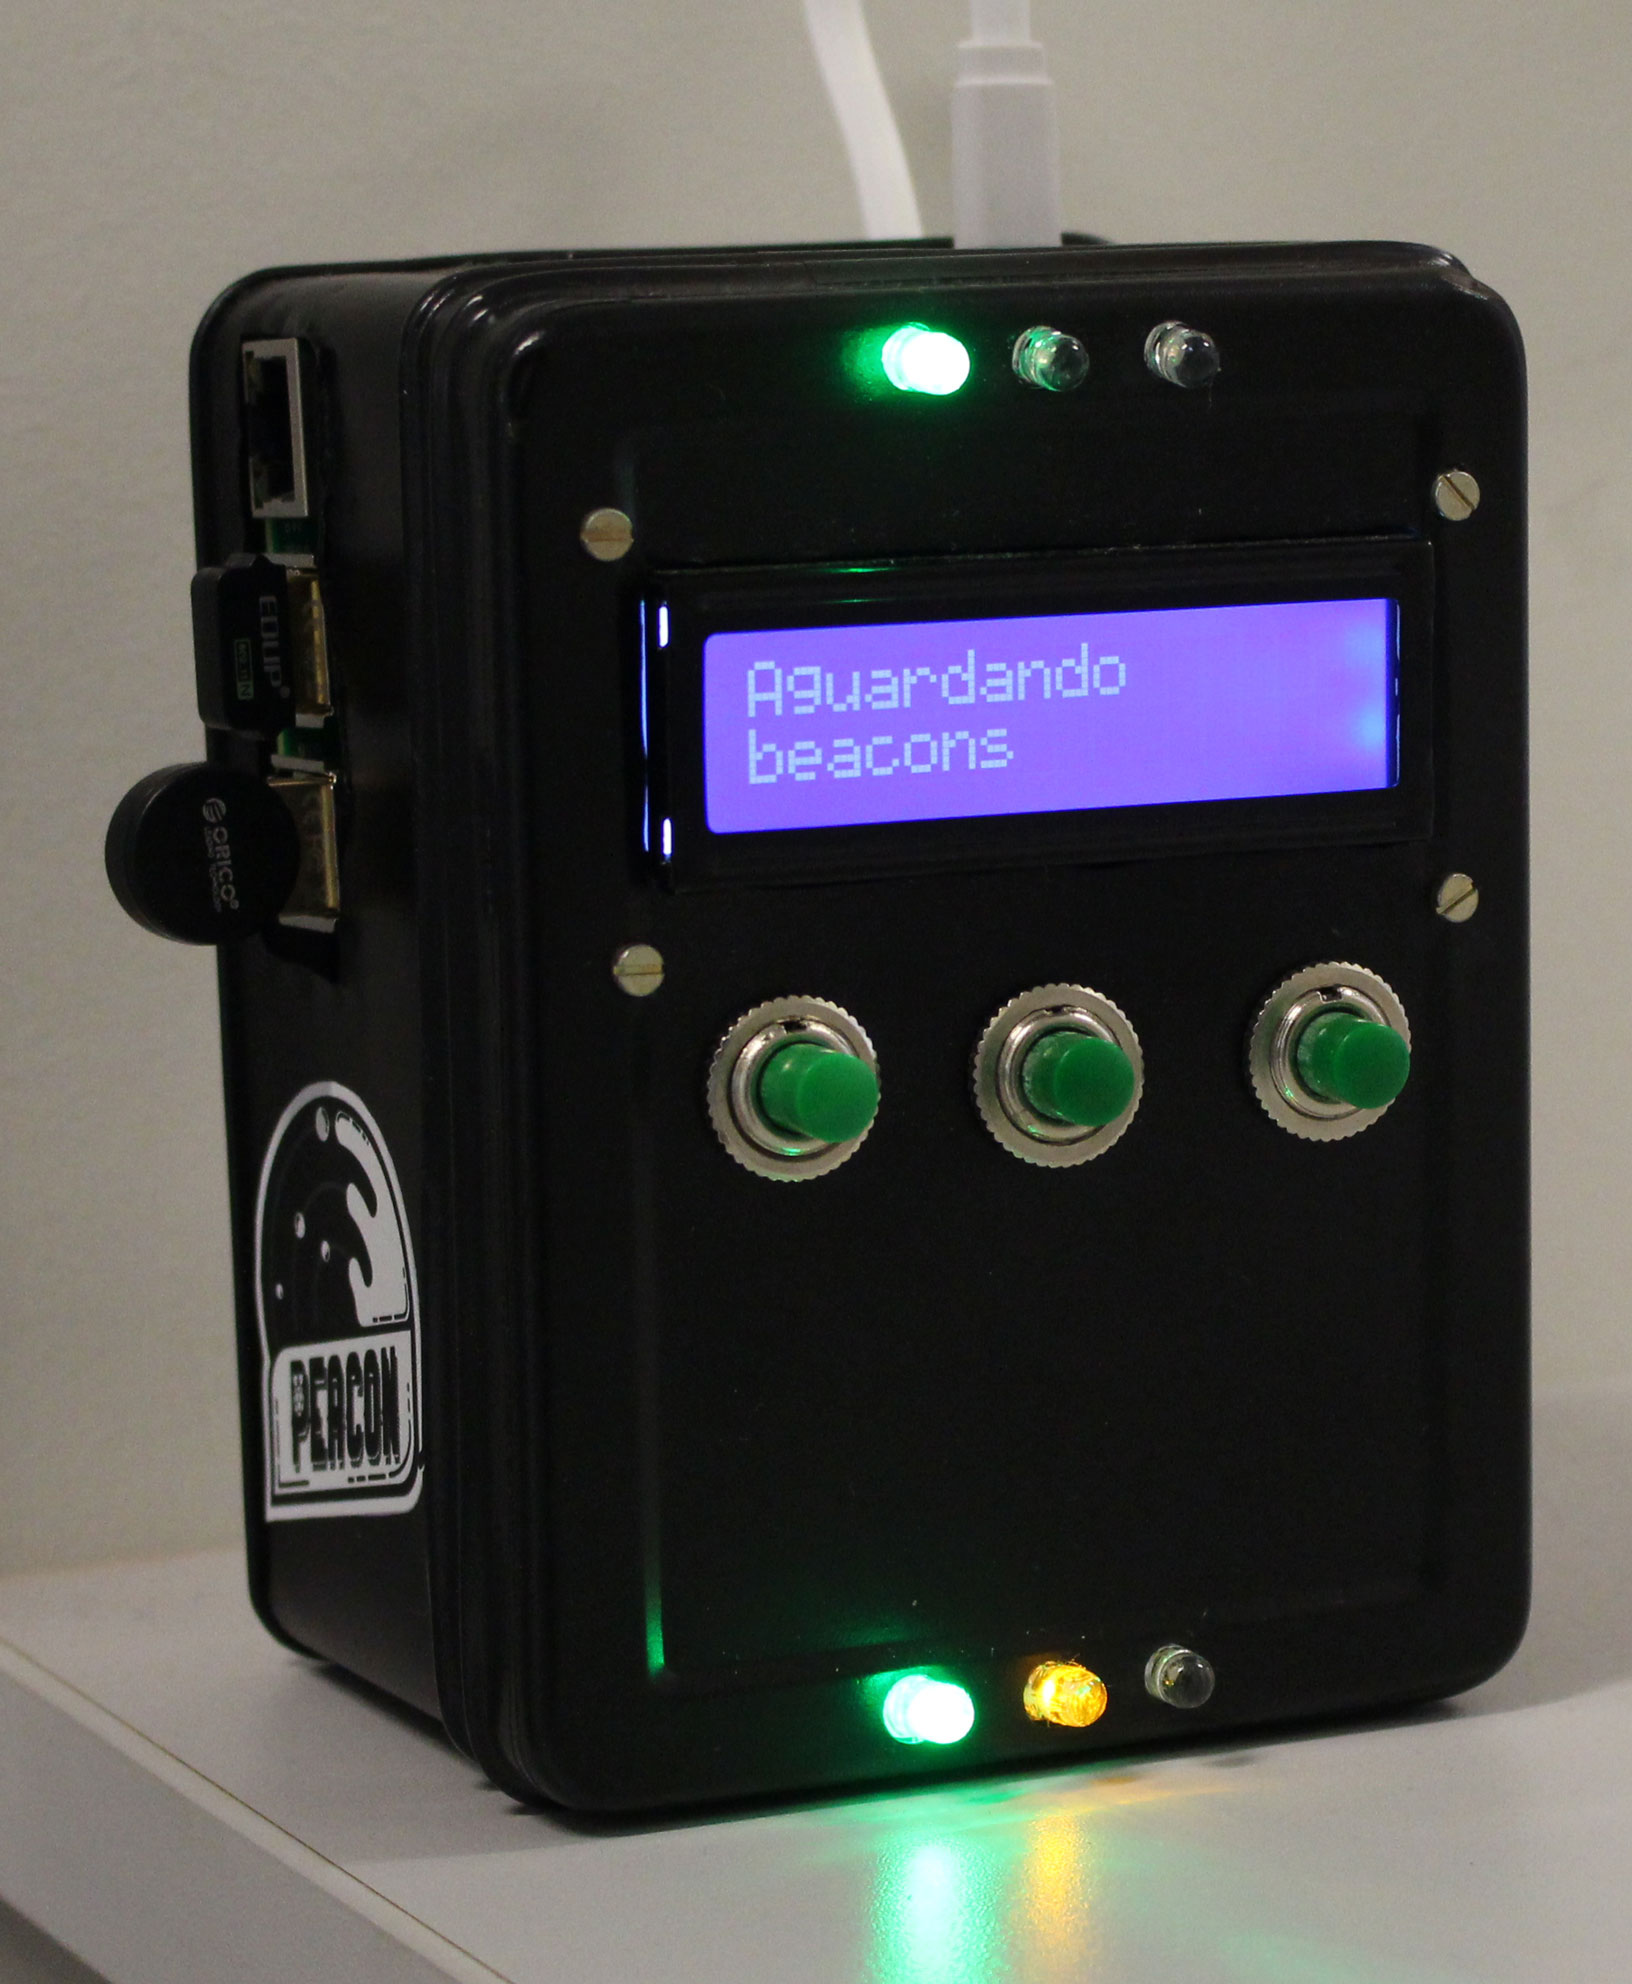
\includegraphics[width=0.65\textwidth]{img/prod-final.jpg}
	\end{center}
	\legend{Fonte: elaborado pelo autor}
\end{figure}

% ----------------------------------------------------------